\documentclass[1p]{elsarticle_modified}
%\bibliographystyle{elsarticle-num}

%\usepackage[colorlinks]{hyperref}
%\usepackage{abbrmath_seonhwa} %\Abb, \Ascr, \Acal ,\Abf, \Afrak
\usepackage{amsfonts}
\usepackage{amssymb}
\usepackage{amsmath}
\usepackage{amsthm}
\usepackage{scalefnt}
\usepackage{amsbsy}
\usepackage{kotex}
\usepackage{caption}
\usepackage{subfig}
\usepackage{color}
\usepackage{graphicx}
\usepackage{xcolor} %% white, black, red, green, blue, cyan, magenta, yellow
\usepackage{float}
\usepackage{setspace}
\usepackage{hyperref}

\usepackage{tikz}
\usetikzlibrary{arrows}

\usepackage{multirow}
\usepackage{array} % fixed length table
\usepackage{hhline}

%%%%%%%%%%%%%%%%%%%%%
\makeatletter
\renewcommand*\env@matrix[1][\arraystretch]{%
	\edef\arraystretch{#1}%
	\hskip -\arraycolsep
	\let\@ifnextchar\new@ifnextchar
	\array{*\c@MaxMatrixCols c}}
\makeatother %https://tex.stackexchange.com/questions/14071/how-can-i-increase-the-line-spacing-in-a-matrix
%%%%%%%%%%%%%%%

\usepackage[normalem]{ulem}

\newcommand{\msout}[1]{\ifmmode\text{\sout{\ensuremath{#1}}}\else\sout{#1}\fi}
%SOURCE: \msout is \stkout macro in https://tex.stackexchange.com/questions/20609/strikeout-in-math-mode

\newcommand{\cancel}[1]{
	\ifmmode
	{\color{red}\msout{#1}}
	\else
	{\color{red}\sout{#1}}
	\fi
}

\newcommand{\add}[1]{
	{\color{blue}\uwave{#1}}
}

\newcommand{\replace}[2]{
	\ifmmode
	{\color{red}\msout{#1}}{\color{blue}\uwave{#2}}
	\else
	{\color{red}\sout{#1}}{\color{blue}\uwave{#2}}
	\fi
}

\newcommand{\Sol}{\mathcal{S}} %segment
\newcommand{\D}{D} %diagram
\newcommand{\A}{\mathcal{A}} %arc


%%%%%%%%%%%%%%%%%%%%%%%%%%%%%5 test

\def\sl{\operatorname{\textup{SL}}(2,\Cbb)}
\def\psl{\operatorname{\textup{PSL}}(2,\Cbb)}
\def\quan{\mkern 1mu \triangleright \mkern 1mu}

\theoremstyle{definition}
\newtheorem{thm}{Theorem}[section]
\newtheorem{prop}[thm]{Proposition}
\newtheorem{lem}[thm]{Lemma}
\newtheorem{ques}[thm]{Question}
\newtheorem{cor}[thm]{Corollary}
\newtheorem{defn}[thm]{Definition}
\newtheorem{exam}[thm]{Example}
\newtheorem{rmk}[thm]{Remark}
\newtheorem{alg}[thm]{Algorithm}

\newcommand{\I}{\sqrt{-1}}
\begin{document}

%\begin{frontmatter}
%
%\title{Boundary parabolic representations of knots up to 8 crossings}
%
%%% Group authors per affiliation:
%\author{Yunhi Cho} 
%\address{Department of Mathematics, University of Seoul, Seoul, Korea}
%\ead{yhcho@uos.ac.kr}
%
%
%\author{Seonhwa Kim} %\fnref{s_kim}}
%\address{Center for Geometry and Physics, Institute for Basic Science, Pohang, 37673, Korea}
%\ead{ryeona17@ibs.re.kr}
%
%\author{Hyuk Kim}
%\address{Department of Mathematical Sciences, Seoul National University, Seoul 08826, Korea}
%\ead{hyukkim@snu.ac.kr}
%
%\author{Seokbeom Yoon}
%\address{Department of Mathematical Sciences, Seoul National University, Seoul, 08826,  Korea}
%\ead{sbyoon15@snu.ac.kr}
%
%\begin{abstract}
%We find all boundary parabolic representation of knots up to 8 crossings.
%
%\end{abstract}
%\begin{keyword}
%    \MSC[2010] 57M25 
%\end{keyword}
%
%\end{frontmatter}

%\linenumbers
%\tableofcontents
%
\newcommand\colored[1]{\textcolor{white}{\rule[-0.35ex]{0.8em}{1.4ex}}\kern-0.8em\color{red} #1}%
%\newcommand\colored[1]{\textcolor{white}{ #1}\kern-2.17ex	\textcolor{white}{ #1}\kern-1.81ex	\textcolor{white}{ #1}\kern-2.15ex\color{red}#1	}

{\Large $\underline{12a_{1067}~(K12a_{1067})}$}

\setlength{\tabcolsep}{10pt}
\renewcommand{\arraystretch}{1.6}
\vspace{1cm}\begin{tabular}{m{100pt}>{\centering\arraybackslash}m{274pt}}
\multirow{5}{120pt}{
	\centering
	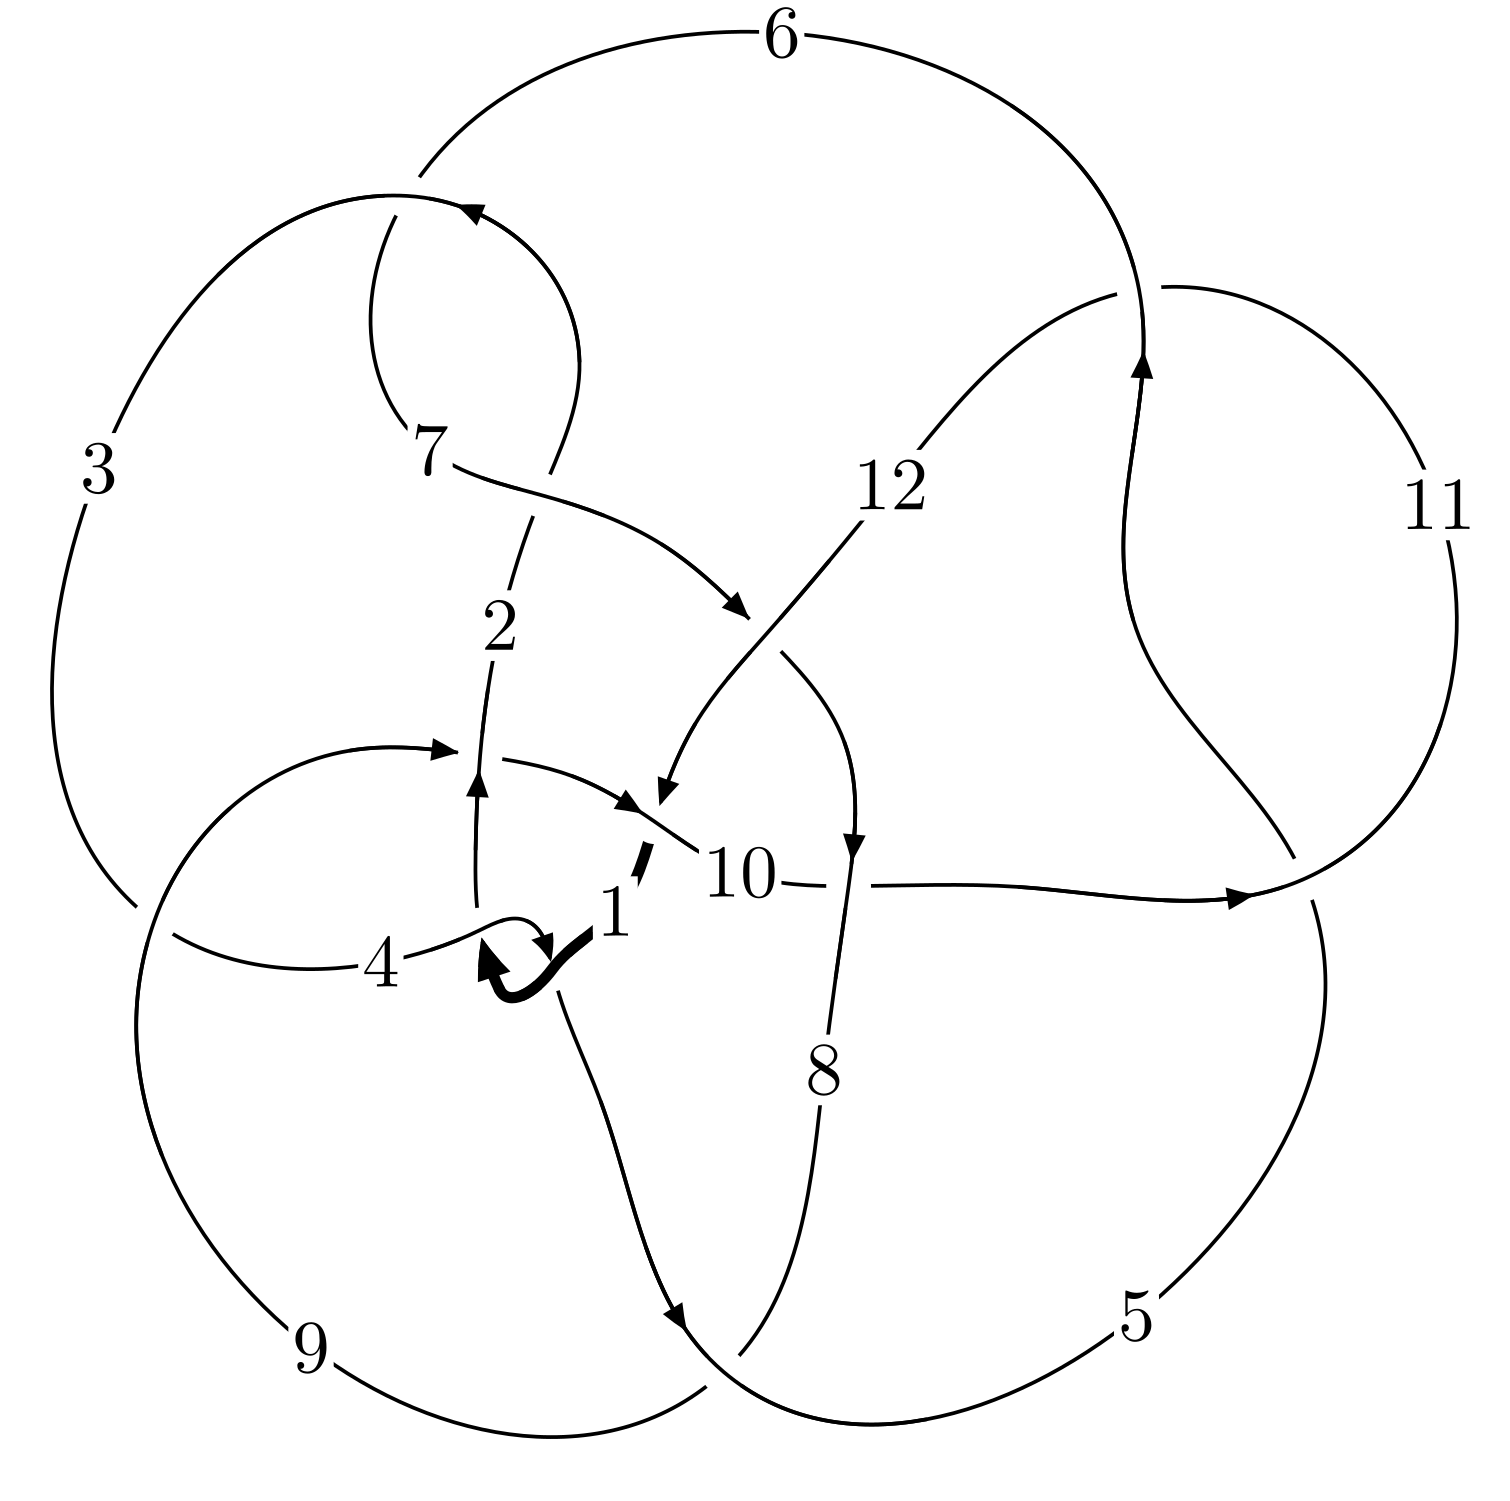
\includegraphics[width=112pt]{../../../GIT/diagram.site/Diagrams/png/1868_12a_1067.png}\\
\ \ \ A knot diagram\footnotemark}&
\allowdisplaybreaks
\textbf{Linearized knot diagam} \\
\cline{2-2}
 &
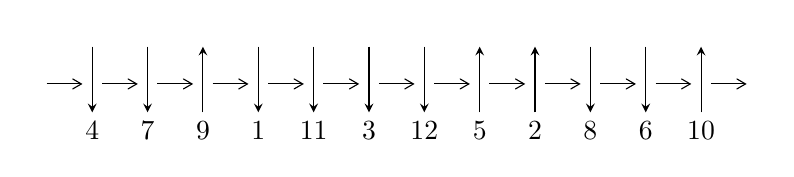
\begin{tikzpicture}[x=20pt, y=17pt]
	% nodes
	\node (C0) at (0, 0) {};
	\node (C1) at (1, 0) {};
	\node (C1U) at (1, +1) {};
	\node (C1D) at (1, -1) {4};

	\node (C2) at (2, 0) {};
	\node (C2U) at (2, +1) {};
	\node (C2D) at (2, -1) {7};

	\node (C3) at (3, 0) {};
	\node (C3U) at (3, +1) {};
	\node (C3D) at (3, -1) {9};

	\node (C4) at (4, 0) {};
	\node (C4U) at (4, +1) {};
	\node (C4D) at (4, -1) {1};

	\node (C5) at (5, 0) {};
	\node (C5U) at (5, +1) {};
	\node (C5D) at (5, -1) {11};

	\node (C6) at (6, 0) {};
	\node (C6U) at (6, +1) {};
	\node (C6D) at (6, -1) {3};

	\node (C7) at (7, 0) {};
	\node (C7U) at (7, +1) {};
	\node (C7D) at (7, -1) {12};

	\node (C8) at (8, 0) {};
	\node (C8U) at (8, +1) {};
	\node (C8D) at (8, -1) {5};

	\node (C9) at (9, 0) {};
	\node (C9U) at (9, +1) {};
	\node (C9D) at (9, -1) {2};

	\node (C10) at (10, 0) {};
	\node (C10U) at (10, +1) {};
	\node (C10D) at (10, -1) {8};

	\node (C11) at (11, 0) {};
	\node (C11U) at (11, +1) {};
	\node (C11D) at (11, -1) {6};

	\node (C12) at (12, 0) {};
	\node (C12U) at (12, +1) {};
	\node (C12D) at (12, -1) {10};
	\node (C13) at (13, 0) {};

	% arrows
	\draw[->,>={angle 60}]
	(C0) edge (C1) (C1) edge (C2) (C2) edge (C3) (C3) edge (C4) (C4) edge (C5) (C5) edge (C6) (C6) edge (C7) (C7) edge (C8) (C8) edge (C9) (C9) edge (C10) (C10) edge (C11) (C11) edge (C12) (C12) edge (C13) ;	\draw[->,>=stealth]
	(C1U) edge (C1D) (C2U) edge (C2D) (C3D) edge (C3U) (C4U) edge (C4D) (C5U) edge (C5D) (C6U) edge (C6D) (C7U) edge (C7D) (C8D) edge (C8U) (C9D) edge (C9U) (C10U) edge (C10D) (C11U) edge (C11D) (C12D) edge (C12U) ;
	\end{tikzpicture} \\
\hhline{~~} \\& 
\textbf{Solving Sequence} \\ \cline{2-2} 
 &
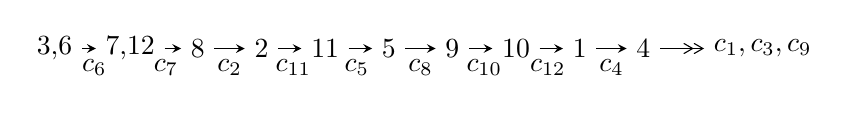
\begin{tikzpicture}[x=23pt, y=7pt]
	% node
	\node (A0) at (-1/8, 0) {3,6};
	\node (A1) at (17/16, 0) {7,12};
	\node (A2) at (17/8, 0) {8};
	\node (A3) at (25/8, 0) {2};
	\node (A4) at (33/8, 0) {11};
	\node (A5) at (41/8, 0) {5};
	\node (A6) at (49/8, 0) {9};
	\node (A7) at (57/8, 0) {10};
	\node (A8) at (65/8, 0) {1};
	\node (A9) at (73/8, 0) {4};
	\node (C1) at (1/2, -1) {$c_{6}$};
	\node (C2) at (13/8, -1) {$c_{7}$};
	\node (C3) at (21/8, -1) {$c_{2}$};
	\node (C4) at (29/8, -1) {$c_{11}$};
	\node (C5) at (37/8, -1) {$c_{5}$};
	\node (C6) at (45/8, -1) {$c_{8}$};
	\node (C7) at (53/8, -1) {$c_{10}$};
	\node (C8) at (61/8, -1) {$c_{12}$};
	\node (C9) at (69/8, -1) {$c_{4}$};
	\node (A10) at (11, 0) {$c_{1},c_{3},c_{9}$};

	% edge
	\draw[->,>=stealth]	
	(A0) edge (A1) (A1) edge (A2) (A2) edge (A3) (A3) edge (A4) (A4) edge (A5) (A5) edge (A6) (A6) edge (A7) (A7) edge (A8) (A8) edge (A9) ;
	\draw[->>,>={angle 60}]	
	(A9) edge (A10);
\end{tikzpicture} \\ 

\end{tabular} \\

\footnotetext{
The image of knot diagram is generated by the software ``\textbf{Draw programme}" developed by Andrew Bartholomew(\url{http://www.layer8.co.uk/maths/draw/index.htm\#Running-draw}), where we modified some parts for our purpose(\url{https://github.com/CATsTAILs/LinksPainter}).
}\phantom \\ \newline 
\centering \textbf{Ideals for irreducible components\footnotemark of $X_{\text{par}}$} 
 
\begin{align*}
I^u_{1}&=\langle 
9.69637\times10^{972} u^{183}+3.83011\times10^{973} u^{182}+\cdots+4.79435\times10^{972} b+4.98318\times10^{972},\\
\phantom{I^u_{1}}&\phantom{= \langle  }3.00989\times10^{973} u^{183}+1.06238\times10^{974} u^{182}+\cdots+9.58869\times10^{972} a-1.13665\times10^{973},\\
\phantom{I^u_{1}}&\phantom{= \langle  }4 u^{184}+18 u^{183}+\cdots- u-1\rangle \\
I^u_{2}&=\langle 
-6.34794\times10^{39} u^{46}+2.02979\times10^{39} u^{45}+\cdots+3.62356\times10^{36} b+1.98963\times10^{38},\\
\phantom{I^u_{2}}&\phantom{= \langle  }-1.15338\times10^{40} u^{46}+4.70729\times10^{39} u^{45}+\cdots+3.62356\times10^{36} a+5.74621\times10^{38},\\
\phantom{I^u_{2}}&\phantom{= \langle  }4 u^{47}-2 u^{46}+\cdots+2 u-1\rangle \\
\\
\end{align*}
\raggedright * 2 irreducible components of $\dim_{\mathbb{C}}=0$, with total 231 representations.\\
\footnotetext{All coefficients of polynomials are rational numbers. But the coefficients are sometimes approximated in decimal forms when there is not enough margin.}
\newpage
\renewcommand{\arraystretch}{1}
\centering \section*{I. $I^u_{1}= \langle 9.70\times10^{972} u^{183}+3.83\times10^{973} u^{182}+\cdots+4.79\times10^{972} b+4.98\times10^{972},\;3.01\times10^{973} u^{183}+1.06\times10^{974} u^{182}+\cdots+9.59\times10^{972} a-1.14\times10^{973},\;4 u^{184}+18 u^{183}+\cdots- u-1 \rangle$}
\flushleft \textbf{(i) Arc colorings}\\
\begin{tabular}{m{7pt} m{180pt} m{7pt} m{180pt} }
\flushright $a_{3}=$&$\begin{pmatrix}0\\u\end{pmatrix}$ \\
\flushright $a_{6}=$&$\begin{pmatrix}1\\0\end{pmatrix}$ \\
\flushright $a_{7}=$&$\begin{pmatrix}1\\u^2\end{pmatrix}$ \\
\flushright $a_{12}=$&$\begin{pmatrix}-3.13900 u^{183}-11.0795 u^{182}+\cdots+11.4796 u+1.18541\\-2.02246 u^{183}-7.98881 u^{182}+\cdots-0.164649 u-1.03939\end{pmatrix}$ \\
\flushright $a_{8}=$&$\begin{pmatrix}-28.3246 u^{183}-115.902 u^{182}+\cdots+0.103156 u+0.195379\\-0.838225 u^{183}-5.38534 u^{182}+\cdots+3.61413 u+1.85430\end{pmatrix}$ \\
\flushright $a_{2}=$&$\begin{pmatrix}u\\u^3+u\end{pmatrix}$ \\
\flushright $a_{11}=$&$\begin{pmatrix}-5.16146 u^{183}-19.0683 u^{182}+\cdots+11.3150 u+0.146023\\-2.02246 u^{183}-7.98881 u^{182}+\cdots-0.164649 u-1.03939\end{pmatrix}$ \\
\flushright $a_{5}=$&$\begin{pmatrix}-2.41286 u^{183}-6.67240 u^{182}+\cdots+7.65328 u-0.944619\\-2.97911 u^{183}-12.4678 u^{182}+\cdots-2.66075 u-1.04249\end{pmatrix}$ \\
\flushright $a_{9}=$&$\begin{pmatrix}0.694380 u^{183}+4.32372 u^{182}+\cdots+26.7412 u-1.97568\\0.884339 u^{183}+4.27172 u^{182}+\cdots+18.5921 u-2.57270\end{pmatrix}$ \\
\flushright $a_{10}=$&$\begin{pmatrix}0.512475 u^{183}+4.12866 u^{182}+\cdots+26.7047 u-2.23706\\0.533045 u^{183}+3.06739 u^{182}+\cdots+18.6661 u-2.67821\end{pmatrix}$ \\
\flushright $a_{1}=$&$\begin{pmatrix}-7.17736 u^{183}-33.1930 u^{182}+\cdots+11.1989 u+15.7224\\-6.39788 u^{183}-28.7785 u^{182}+\cdots+10.4754 u+5.75485\end{pmatrix}$ \\
\flushright $a_{4}=$&$\begin{pmatrix}11.8637 u^{183}+48.5407 u^{182}+\cdots-47.3080 u+4.31958\\5.27352 u^{183}+21.4561 u^{182}+\cdots-25.8612 u+1.42500\end{pmatrix}$\\&\end{tabular}
\flushleft \textbf{(ii) Obstruction class $= -1$}\\~\\
\flushleft \textbf{(iii) Cusp Shapes $= 4.22703 u^{183}+16.2157 u^{182}+\cdots-63.6205 u-1.32587$}\\~\\
\newpage\renewcommand{\arraystretch}{1}
\flushleft \textbf{(iv) u-Polynomials at the component}\newline \\
\begin{tabular}{m{50pt}|m{274pt}}
Crossings & \hspace{64pt}u-Polynomials at each crossing \\
\hline $$\begin{aligned}c_{1},c_{4}\end{aligned}$$&$\begin{aligned}
&u^{184}-6 u^{183}+\cdots-249 u+23
\end{aligned}$\\
\hline $$\begin{aligned}c_{2},c_{6}\end{aligned}$$&$\begin{aligned}
&4(4 u^{184}+18 u^{183}+\cdots- u-1)
\end{aligned}$\\
\hline $$\begin{aligned}c_{3}\end{aligned}$$&$\begin{aligned}
&4(4 u^{184}+10 u^{183}+\cdots+6499876 u-332573)
\end{aligned}$\\
\hline $$\begin{aligned}c_{5},c_{11}\end{aligned}$$&$\begin{aligned}
&u^{184}-5 u^{183}+\cdots-626819 u-61241
\end{aligned}$\\
\hline $$\begin{aligned}c_{7}\end{aligned}$$&$\begin{aligned}
&u^{184}+3 u^{183}+\cdots-584840944 u+146659264
\end{aligned}$\\
\hline $$\begin{aligned}c_{8}\end{aligned}$$&$\begin{aligned}
&u^{184}-7 u^{183}+\cdots-15606197942 u-994895348
\end{aligned}$\\
\hline $$\begin{aligned}c_{9}\end{aligned}$$&$\begin{aligned}
&4(4 u^{184}-6 u^{183}+\cdots+64953 u+127)
\end{aligned}$\\
\hline $$\begin{aligned}c_{10}\end{aligned}$$&$\begin{aligned}
&16(16 u^{184}+372 u^{183}+\cdots+2.52928\times10^{7} u+2248063)
\end{aligned}$\\
\hline $$\begin{aligned}c_{12}\end{aligned}$$&$\begin{aligned}
&u^{184}+15 u^{183}+\cdots+3307328 u+94624
\end{aligned}$\\
\hline
\end{tabular}\\~\\
\newpage\renewcommand{\arraystretch}{1}
\flushleft \textbf{(v) Riley Polynomials at the component}\newline \\
\begin{tabular}{m{50pt}|m{274pt}}
Crossings & \hspace{64pt}Riley Polynomials at each crossing \\
\hline $$\begin{aligned}c_{1},c_{4}\end{aligned}$$&$\begin{aligned}
&y^{184}+112 y^{183}+\cdots+67259 y+529
\end{aligned}$\\
\hline $$\begin{aligned}c_{2},c_{6}\end{aligned}$$&$\begin{aligned}
&16(16 y^{184}+1444 y^{183}+\cdots+75 y+1)
\end{aligned}$\\
\hline $$\begin{aligned}c_{3}\end{aligned}$$&$\begin{aligned}
&16(16 y^{184}+164 y^{183}+\cdots-4.68138\times10^{12} y+1.10605\times10^{11})
\end{aligned}$\\
\hline $$\begin{aligned}c_{5},c_{11}\end{aligned}$$&$\begin{aligned}
&y^{184}-121 y^{183}+\cdots+83127663735 y+3750460081
\end{aligned}$\\
\hline $$\begin{aligned}c_{7}\end{aligned}$$&$\begin{aligned}
&y^{184}-59 y^{183}+\cdots-2085041048441058048 y+21508939717021696
\end{aligned}$\\
\hline $$\begin{aligned}c_{8}\end{aligned}$$&$\begin{aligned}
&y^{184}+67 y^{183}+\cdots+1.72\times10^{19} y+9.90\times10^{17}
\end{aligned}$\\
\hline $$\begin{aligned}c_{9}\end{aligned}$$&$\begin{aligned}
&16(16 y^{184}-60 y^{183}+\cdots-4.55483\times10^{9} y+16129)
\end{aligned}$\\
\hline $$\begin{aligned}c_{10}\end{aligned}$$&$\begin{aligned}
&256\\
&\cdot(256 y^{184}-9328 y^{183}+\cdots-317358447741910 y+5053787251969)
\end{aligned}$\\
\hline $$\begin{aligned}c_{12}\end{aligned}$$&$\begin{aligned}
&y^{184}+5 y^{183}+\cdots+1539978428928 y+8953701376
\end{aligned}$\\
\hline
\end{tabular}\\~\\
\newpage\flushleft \textbf{(vi) Complex Volumes and Cusp Shapes}
$$\begin{array}{c|c|c}  
\text{Solutions to }I^u_{1}& \I (\text{vol} + \sqrt{-1}CS) & \text{Cusp shape}\\
 \hline 
\begin{aligned}
u &= -0.408140 + 0.919874 I \\
a &= \phantom{-}0.468378 + 0.427870 I \\
b &= \phantom{-}1.51005 + 0.08124 I\end{aligned}
 & -1.37864 - 2.50987 I & \phantom{-0.000000 } 0 \\ \hline\begin{aligned}
u &= -0.408140 - 0.919874 I \\
a &= \phantom{-}0.468378 - 0.427870 I \\
b &= \phantom{-}1.51005 - 0.08124 I\end{aligned}
 & -1.37864 + 2.50987 I & \phantom{-0.000000 } 0 \\ \hline\begin{aligned}
u &= \phantom{-}0.347511 + 0.928057 I \\
a &= -0.24952 + 1.41068 I \\
b &= \phantom{-}0.187116 - 0.192914 I\end{aligned}
 & \phantom{-}0.71096 - 4.45447 I & \phantom{-0.000000 } 0 \\ \hline\begin{aligned}
u &= \phantom{-}0.347511 - 0.928057 I \\
a &= -0.24952 - 1.41068 I \\
b &= \phantom{-}0.187116 + 0.192914 I\end{aligned}
 & \phantom{-}0.71096 + 4.45447 I & \phantom{-0.000000 } 0 \\ \hline\begin{aligned}
u &= \phantom{-}0.414485 + 0.922428 I \\
a &= -0.74768 + 1.57493 I \\
b &= \phantom{-}0.325405 - 1.011900 I\end{aligned}
 & \phantom{-}0.81162 - 5.05777 I & \phantom{-0.000000 } 0 \\ \hline\begin{aligned}
u &= \phantom{-}0.414485 - 0.922428 I \\
a &= -0.74768 - 1.57493 I \\
b &= \phantom{-}0.325405 + 1.011900 I\end{aligned}
 & \phantom{-}0.81162 + 5.05777 I & \phantom{-0.000000 } 0 \\ \hline\begin{aligned}
u &= \phantom{-}0.936267 + 0.290628 I \\
a &= \phantom{-}0.723436 - 0.270809 I \\
b &= -0.018333 + 0.974541 I\end{aligned}
 & \phantom{-}0.70461 + 9.22244 I & \phantom{-0.000000 } 0 \\ \hline\begin{aligned}
u &= \phantom{-}0.936267 - 0.290628 I \\
a &= \phantom{-}0.723436 + 0.270809 I \\
b &= -0.018333 - 0.974541 I\end{aligned}
 & \phantom{-}0.70461 - 9.22244 I & \phantom{-0.000000 } 0 \\ \hline\begin{aligned}
u &= -0.389627 + 0.897196 I \\
a &= -0.82128 - 1.61223 I \\
b &= \phantom{-}0.172816 + 1.211310 I\end{aligned}
 & \phantom{-}0.39458 + 1.97082 I & \phantom{-0.000000 } 0 \\ \hline\begin{aligned}
u &= -0.389627 - 0.897196 I \\
a &= -0.82128 + 1.61223 I \\
b &= \phantom{-}0.172816 - 1.211310 I\end{aligned}
 & \phantom{-}0.39458 - 1.97082 I & \phantom{-0.000000 } 0\\
 \hline 
 \end{array}$$\newpage$$\begin{array}{c|c|c}  
\text{Solutions to }I^u_{1}& \I (\text{vol} + \sqrt{-1}CS) & \text{Cusp shape}\\
 \hline 
\begin{aligned}
u &= \phantom{-}0.386856 + 0.946622 I \\
a &= -0.55309 + 1.52788 I \\
b &= \phantom{-}0.223782 - 0.579332 I\end{aligned}
 & \phantom{-}0.71363 - 4.10768 I & \phantom{-0.000000 } 0 \\ \hline\begin{aligned}
u &= \phantom{-}0.386856 - 0.946622 I \\
a &= -0.55309 - 1.52788 I \\
b &= \phantom{-}0.223782 + 0.579332 I\end{aligned}
 & \phantom{-}0.71363 + 4.10768 I & \phantom{-0.000000 } 0 \\ \hline\begin{aligned}
u &= -0.598540 + 0.840118 I \\
a &= -1.00327 - 1.66735 I \\
b &= -0.835767 + 0.193058 I\end{aligned}
 & \phantom{-}2.88033 + 5.29178 I & \phantom{-0.000000 } 0 \\ \hline\begin{aligned}
u &= -0.598540 - 0.840118 I \\
a &= -1.00327 + 1.66735 I \\
b &= -0.835767 - 0.193058 I\end{aligned}
 & \phantom{-}2.88033 - 5.29178 I & \phantom{-0.000000 } 0 \\ \hline\begin{aligned}
u &= \phantom{-}0.387149 + 0.886872 I \\
a &= -1.65326 + 1.80661 I \\
b &= \phantom{-}0.15896 - 2.04360 I\end{aligned}
 & \phantom{-}6.92848 - 1.61446 I & \phantom{-0.000000 } 0 \\ \hline\begin{aligned}
u &= \phantom{-}0.387149 - 0.886872 I \\
a &= -1.65326 - 1.80661 I \\
b &= \phantom{-}0.15896 + 2.04360 I\end{aligned}
 & \phantom{-}6.92848 + 1.61446 I & \phantom{-0.000000 } 0 \\ \hline\begin{aligned}
u &= -0.397961 + 0.970113 I \\
a &= -0.52923 - 1.79836 I \\
b &= -0.403072 + 0.707760 I\end{aligned}
 & \phantom{-}3.06213 + 5.71906 I & \phantom{-0.000000 } 0 \\ \hline\begin{aligned}
u &= -0.397961 - 0.970113 I \\
a &= -0.52923 + 1.79836 I \\
b &= -0.403072 - 0.707760 I\end{aligned}
 & \phantom{-}3.06213 - 5.71906 I & \phantom{-0.000000 } 0 \\ \hline\begin{aligned}
u &= -0.362407 + 0.869445 I \\
a &= -0.75689 - 1.30416 I \\
b &= \phantom{-}0.336318 + 1.211430 I\end{aligned}
 & \phantom{-}0.250731 + 1.210620 I & \phantom{-0.000000 } 0 \\ \hline\begin{aligned}
u &= -0.362407 - 0.869445 I \\
a &= -0.75689 + 1.30416 I \\
b &= \phantom{-}0.336318 - 1.211430 I\end{aligned}
 & \phantom{-}0.250731 - 1.210620 I & \phantom{-0.000000 } 0\\
 \hline 
 \end{array}$$\newpage$$\begin{array}{c|c|c}  
\text{Solutions to }I^u_{1}& \I (\text{vol} + \sqrt{-1}CS) & \text{Cusp shape}\\
 \hline 
\begin{aligned}
u &= -0.430135 + 0.978941 I \\
a &= -0.70095 - 1.39377 I \\
b &= \phantom{-}0.688817 + 0.707721 I\end{aligned}
 & \phantom{-}4.26154 + 6.12115 I & \phantom{-0.000000 } 0 \\ \hline\begin{aligned}
u &= -0.430135 - 0.978941 I \\
a &= -0.70095 + 1.39377 I \\
b &= \phantom{-}0.688817 - 0.707721 I\end{aligned}
 & \phantom{-}4.26154 - 6.12115 I & \phantom{-0.000000 } 0 \\ \hline\begin{aligned}
u &= \phantom{-}0.923728 + 0.035921 I \\
a &= \phantom{-}0.784119 + 0.058833 I \\
b &= -0.065795 - 0.428784 I\end{aligned}
 & \phantom{-}0.08718 + 4.16864 I & \phantom{-0.000000 } 0 \\ \hline\begin{aligned}
u &= \phantom{-}0.923728 - 0.035921 I \\
a &= \phantom{-}0.784119 - 0.058833 I \\
b &= -0.065795 + 0.428784 I\end{aligned}
 & \phantom{-}0.08718 - 4.16864 I & \phantom{-0.000000 } 0 \\ \hline\begin{aligned}
u &= \phantom{-}0.281847 + 1.038920 I \\
a &= \phantom{-}0.950210 - 0.904620 I \\
b &= -0.526128 + 0.721953 I\end{aligned}
 & \phantom{-}3.42270 - 0.97311 I & \phantom{-0.000000 } 0 \\ \hline\begin{aligned}
u &= \phantom{-}0.281847 - 1.038920 I \\
a &= \phantom{-}0.950210 + 0.904620 I \\
b &= -0.526128 - 0.721953 I\end{aligned}
 & \phantom{-}3.42270 + 0.97311 I & \phantom{-0.000000 } 0 \\ \hline\begin{aligned}
u &= -0.314115 + 1.036040 I \\
a &= -0.900858 - 0.166185 I \\
b &= \phantom{-}1.080560 + 0.729888 I\end{aligned}
 & \phantom{-}2.58839 - 3.79400 I & \phantom{-0.000000 } 0 \\ \hline\begin{aligned}
u &= -0.314115 - 1.036040 I \\
a &= -0.900858 + 0.166185 I \\
b &= \phantom{-}1.080560 - 0.729888 I\end{aligned}
 & \phantom{-}2.58839 + 3.79400 I & \phantom{-0.000000 } 0 \\ \hline\begin{aligned}
u &= -0.169340 + 1.072090 I \\
a &= -0.522139 - 0.399251 I \\
b &= \phantom{-}0.643915 - 0.083937 I\end{aligned}
 & -0.103146 + 1.087630 I & \phantom{-0.000000 } 0 \\ \hline\begin{aligned}
u &= -0.169340 - 1.072090 I \\
a &= -0.522139 + 0.399251 I \\
b &= \phantom{-}0.643915 + 0.083937 I\end{aligned}
 & -0.103146 - 1.087630 I & \phantom{-0.000000 } 0\\
 \hline 
 \end{array}$$\newpage$$\begin{array}{c|c|c}  
\text{Solutions to }I^u_{1}& \I (\text{vol} + \sqrt{-1}CS) & \text{Cusp shape}\\
 \hline 
\begin{aligned}
u &= \phantom{-}1.026900 + 0.396959 I \\
a &= -0.946965 - 0.259094 I \\
b &= -1.052410 - 0.095352 I\end{aligned}
 & -4.26445 - 3.56478 I & \phantom{-0.000000 } 0 \\ \hline\begin{aligned}
u &= \phantom{-}1.026900 - 0.396959 I \\
a &= -0.946965 + 0.259094 I \\
b &= -1.052410 + 0.095352 I\end{aligned}
 & -4.26445 + 3.56478 I & \phantom{-0.000000 } 0 \\ \hline\begin{aligned}
u &= -0.505306 + 0.978686 I \\
a &= -0.505234 + 0.189205 I \\
b &= \phantom{-}1.68157 + 0.48204 I\end{aligned}
 & -1.95917 + 7.82733 I & \phantom{-0.000000 } 0 \\ \hline\begin{aligned}
u &= -0.505306 - 0.978686 I \\
a &= -0.505234 - 0.189205 I \\
b &= \phantom{-}1.68157 - 0.48204 I\end{aligned}
 & -1.95917 - 7.82733 I & \phantom{-0.000000 } 0 \\ \hline\begin{aligned}
u &= \phantom{-}0.528603 + 0.971751 I \\
a &= -0.267204 - 0.043964 I \\
b &= \phantom{-}1.57732 - 0.43029 I\end{aligned}
 & -5.82786 - 2.25349 I & \phantom{-0.000000 } 0 \\ \hline\begin{aligned}
u &= \phantom{-}0.528603 - 0.971751 I \\
a &= -0.267204 + 0.043964 I \\
b &= \phantom{-}1.57732 + 0.43029 I\end{aligned}
 & -5.82786 + 2.25349 I & \phantom{-0.000000 } 0 \\ \hline\begin{aligned}
u &= -0.371982 + 1.043230 I \\
a &= \phantom{-}1.00034 + 1.02546 I \\
b &= -0.420802 - 0.873508 I\end{aligned}
 & \phantom{-}3.44755 + 0.37029 I & \phantom{-0.000000 } 0 \\ \hline\begin{aligned}
u &= -0.371982 - 1.043230 I \\
a &= \phantom{-}1.00034 - 1.02546 I \\
b &= -0.420802 + 0.873508 I\end{aligned}
 & \phantom{-}3.44755 - 0.37029 I & \phantom{-0.000000 } 0 \\ \hline\begin{aligned}
u &= -0.969711 + 0.536288 I \\
a &= \phantom{-}0.076731 - 0.456367 I \\
b &= -1.082330 - 0.371542 I\end{aligned}
 & -4.27619 + 1.85568 I & \phantom{-0.000000 } 0 \\ \hline\begin{aligned}
u &= -0.969711 - 0.536288 I \\
a &= \phantom{-}0.076731 + 0.456367 I \\
b &= -1.082330 + 0.371542 I\end{aligned}
 & -4.27619 - 1.85568 I & \phantom{-0.000000 } 0\\
 \hline 
 \end{array}$$\newpage$$\begin{array}{c|c|c}  
\text{Solutions to }I^u_{1}& \I (\text{vol} + \sqrt{-1}CS) & \text{Cusp shape}\\
 \hline 
\begin{aligned}
u &= -1.061950 + 0.322851 I \\
a &= \phantom{-}0.676768 + 0.257664 I \\
b &= \phantom{-}0.058107 - 0.961838 I\end{aligned}
 & -3.14855 - 2.88375 I & \phantom{-0.000000 } 0 \\ \hline\begin{aligned}
u &= -1.061950 - 0.322851 I \\
a &= \phantom{-}0.676768 - 0.257664 I \\
b &= \phantom{-}0.058107 + 0.961838 I\end{aligned}
 & -3.14855 + 2.88375 I & \phantom{-0.000000 } 0 \\ \hline\begin{aligned}
u &= -0.450313 + 1.028690 I \\
a &= \phantom{-}1.75389 + 0.84402 I \\
b &= \phantom{-}1.241200 - 0.130319 I\end{aligned}
 & -0.17468 + 10.02130 I & \phantom{-0.000000 } 0 \\ \hline\begin{aligned}
u &= -0.450313 - 1.028690 I \\
a &= \phantom{-}1.75389 - 0.84402 I \\
b &= \phantom{-}1.241200 + 0.130319 I\end{aligned}
 & -0.17468 - 10.02130 I & \phantom{-0.000000 } 0 \\ \hline\begin{aligned}
u &= \phantom{-}0.419405 + 1.048920 I \\
a &= \phantom{-}1.55024 - 0.23042 I \\
b &= \phantom{-}1.300290 + 0.017985 I\end{aligned}
 & -4.53117 - 3.67527 I & \phantom{-0.000000 } 0 \\ \hline\begin{aligned}
u &= \phantom{-}0.419405 - 1.048920 I \\
a &= \phantom{-}1.55024 + 0.23042 I \\
b &= \phantom{-}1.300290 - 0.017985 I\end{aligned}
 & -4.53117 + 3.67527 I & \phantom{-0.000000 } 0 \\ \hline\begin{aligned}
u &= -0.561516 + 0.982387 I \\
a &= \phantom{-}1.09147 + 0.98522 I \\
b &= \phantom{-}1.032500 - 0.173802 I\end{aligned}
 & \phantom{-}3.47444 - 0.63871 I & \phantom{-0.000000 } 0 \\ \hline\begin{aligned}
u &= -0.561516 - 0.982387 I \\
a &= \phantom{-}1.09147 - 0.98522 I \\
b &= \phantom{-}1.032500 + 0.173802 I\end{aligned}
 & \phantom{-}3.47444 + 0.63871 I & \phantom{-0.000000 } 0 \\ \hline\begin{aligned}
u &= \phantom{-}0.333214 + 0.786452 I \\
a &= -0.186114 + 1.268040 I \\
b &= \phantom{-}0.153328 - 0.956820 I\end{aligned}
 & \phantom{-}0.28532 + 1.75546 I & \phantom{-0.000000 } 0 \\ \hline\begin{aligned}
u &= \phantom{-}0.333214 - 0.786452 I \\
a &= -0.186114 - 1.268040 I \\
b &= \phantom{-}0.153328 + 0.956820 I\end{aligned}
 & \phantom{-}0.28532 - 1.75546 I & \phantom{-0.000000 } 0\\
 \hline 
 \end{array}$$\newpage$$\begin{array}{c|c|c}  
\text{Solutions to }I^u_{1}& \I (\text{vol} + \sqrt{-1}CS) & \text{Cusp shape}\\
 \hline 
\begin{aligned}
u &= -0.889487 + 0.746374 I \\
a &= \phantom{-}0.293423 - 0.103625 I \\
b &= \phantom{-}1.35003 + 0.43451 I\end{aligned}
 & -0.40458 - 2.51278 I & \phantom{-0.000000 } 0 \\ \hline\begin{aligned}
u &= -0.889487 - 0.746374 I \\
a &= \phantom{-}0.293423 + 0.103625 I \\
b &= \phantom{-}1.35003 - 0.43451 I\end{aligned}
 & -0.40458 + 2.51278 I & \phantom{-0.000000 } 0 \\ \hline\begin{aligned}
u &= \phantom{-}0.647529 + 0.968786 I \\
a &= \phantom{-}0.912059 - 1.075660 I \\
b &= \phantom{-}0.326805 + 1.263330 I\end{aligned}
 & \phantom{-}5.12494 - 2.86592 I & \phantom{-0.000000 } 0 \\ \hline\begin{aligned}
u &= \phantom{-}0.647529 - 0.968786 I \\
a &= \phantom{-}0.912059 + 1.075660 I \\
b &= \phantom{-}0.326805 - 1.263330 I\end{aligned}
 & \phantom{-}5.12494 + 2.86592 I & \phantom{-0.000000 } 0 \\ \hline\begin{aligned}
u &= \phantom{-}0.521786 + 0.651265 I \\
a &= -0.08453 + 2.96521 I \\
b &= -1.261640 - 0.574391 I\end{aligned}
 & -6.84437 - 2.04453 I & \phantom{-0.000000 } 0 \\ \hline\begin{aligned}
u &= \phantom{-}0.521786 - 0.651265 I \\
a &= -0.08453 - 2.96521 I \\
b &= -1.261640 + 0.574391 I\end{aligned}
 & -6.84437 + 2.04453 I & \phantom{-0.000000 } 0 \\ \hline\begin{aligned}
u &= -0.488376 + 0.666176 I \\
a &= -0.04949 - 2.88367 I \\
b &= -1.35023 + 0.61079 I\end{aligned}
 & -2.97063 - 3.72020 I & \phantom{-0.000000 } 0 \\ \hline\begin{aligned}
u &= -0.488376 - 0.666176 I \\
a &= -0.04949 + 2.88367 I \\
b &= -1.35023 - 0.61079 I\end{aligned}
 & -2.97063 + 3.72020 I & \phantom{-0.000000 } 0 \\ \hline\begin{aligned}
u &= \phantom{-}0.153872 + 1.164880 I \\
a &= -0.23785 + 1.46858 I \\
b &= -0.509986 - 0.890790 I\end{aligned}
 & \phantom{-}8.65940 - 4.16811 I & \phantom{-0.000000 } 0 \\ \hline\begin{aligned}
u &= \phantom{-}0.153872 - 1.164880 I \\
a &= -0.23785 - 1.46858 I \\
b &= -0.509986 + 0.890790 I\end{aligned}
 & \phantom{-}8.65940 + 4.16811 I & \phantom{-0.000000 } 0\\
 \hline 
 \end{array}$$\newpage$$\begin{array}{c|c|c}  
\text{Solutions to }I^u_{1}& \I (\text{vol} + \sqrt{-1}CS) & \text{Cusp shape}\\
 \hline 
\begin{aligned}
u &= \phantom{-}0.577567 + 0.582303 I \\
a &= \phantom{-}0.715962 + 0.008979 I \\
b &= \phantom{-}0.765651 - 0.083496 I\end{aligned}
 & -0.042971 + 1.173170 I & \phantom{-0.000000 } 0 \\ \hline\begin{aligned}
u &= \phantom{-}0.577567 - 0.582303 I \\
a &= \phantom{-}0.715962 - 0.008979 I \\
b &= \phantom{-}0.765651 + 0.083496 I\end{aligned}
 & -0.042971 - 1.173170 I & \phantom{-0.000000 } 0 \\ \hline\begin{aligned}
u &= -0.534355 + 1.053900 I \\
a &= \phantom{-}0.03926 + 1.88650 I \\
b &= \phantom{-}1.59638 - 0.62647 I\end{aligned}
 & \phantom{-}1.18807 + 10.41070 I & \phantom{-0.000000 } 0 \\ \hline\begin{aligned}
u &= -0.534355 - 1.053900 I \\
a &= \phantom{-}0.03926 - 1.88650 I \\
b &= \phantom{-}1.59638 + 0.62647 I\end{aligned}
 & \phantom{-}1.18807 - 10.41070 I & \phantom{-0.000000 } 0 \\ \hline\begin{aligned}
u &= \phantom{-}0.060532 + 0.812643 I \\
a &= \phantom{-}0.040796 + 0.208195 I \\
b &= \phantom{-}0.410695 - 0.434856 I\end{aligned}
 & -0.214445 + 1.140940 I & \phantom{-0.000000 } 0 \\ \hline\begin{aligned}
u &= \phantom{-}0.060532 - 0.812643 I \\
a &= \phantom{-}0.040796 - 0.208195 I \\
b &= \phantom{-}0.410695 + 0.434856 I\end{aligned}
 & -0.214445 - 1.140940 I & \phantom{-0.000000 } 0 \\ \hline\begin{aligned}
u &= -0.536394 + 0.594861 I \\
a &= \phantom{-}0.00338 - 3.29524 I \\
b &= -1.123240 + 0.533124 I\end{aligned}
 & -2.22105 + 7.91268 I & \phantom{-0.000000 } 0 \\ \hline\begin{aligned}
u &= -0.536394 - 0.594861 I \\
a &= \phantom{-}0.00338 + 3.29524 I \\
b &= -1.123240 - 0.533124 I\end{aligned}
 & -2.22105 - 7.91268 I & \phantom{-0.000000 } 0 \\ \hline\begin{aligned}
u &= \phantom{-}0.552591 + 1.066900 I \\
a &= -0.32386 + 1.72792 I \\
b &= -0.998874 - 0.566217 I\end{aligned}
 & \phantom{-}1.68114 - 5.76963 I & \phantom{-0.000000 } 0 \\ \hline\begin{aligned}
u &= \phantom{-}0.552591 - 1.066900 I \\
a &= -0.32386 - 1.72792 I \\
b &= -0.998874 + 0.566217 I\end{aligned}
 & \phantom{-}1.68114 + 5.76963 I & \phantom{-0.000000 } 0\\
 \hline 
 \end{array}$$\newpage$$\begin{array}{c|c|c}  
\text{Solutions to }I^u_{1}& \I (\text{vol} + \sqrt{-1}CS) & \text{Cusp shape}\\
 \hline 
\begin{aligned}
u &= -0.522020 + 1.097030 I \\
a &= \phantom{-}0.225988 - 0.639916 I \\
b &= \phantom{-}1.344370 + 0.357098 I\end{aligned}
 & -0.64833 - 3.45209 I & \phantom{-0.000000 } 0 \\ \hline\begin{aligned}
u &= -0.522020 - 1.097030 I \\
a &= \phantom{-}0.225988 + 0.639916 I \\
b &= \phantom{-}1.344370 - 0.357098 I\end{aligned}
 & -0.64833 + 3.45209 I & \phantom{-0.000000 } 0 \\ \hline\begin{aligned}
u &= \phantom{-}0.020334 + 1.217110 I \\
a &= \phantom{-}0.042520 - 1.264440 I \\
b &= -0.479190 + 0.852671 I\end{aligned}
 & \phantom{-}3.97797 + 0.31674 I & \phantom{-0.000000 } 0 \\ \hline\begin{aligned}
u &= \phantom{-}0.020334 - 1.217110 I \\
a &= \phantom{-}0.042520 + 1.264440 I \\
b &= -0.479190 - 0.852671 I\end{aligned}
 & \phantom{-}3.97797 - 0.31674 I & \phantom{-0.000000 } 0 \\ \hline\begin{aligned}
u &= \phantom{-}0.515416 + 1.105500 I \\
a &= -0.20876 - 1.98005 I \\
b &= \phantom{-}1.44543 + 0.41988 I\end{aligned}
 & -2.63137 - 10.17830 I & \phantom{-0.000000 } 0 \\ \hline\begin{aligned}
u &= \phantom{-}0.515416 - 1.105500 I \\
a &= -0.20876 + 1.98005 I \\
b &= \phantom{-}1.44543 - 0.41988 I\end{aligned}
 & -2.63137 + 10.17830 I & \phantom{-0.000000 } 0 \\ \hline\begin{aligned}
u &= \phantom{-}0.693865 + 0.355004 I \\
a &= -0.099338 + 0.657177 I \\
b &= -1.346610 + 0.340925 I\end{aligned}
 & -5.33037 + 3.15613 I & \phantom{-0.000000 } 0 \\ \hline\begin{aligned}
u &= \phantom{-}0.693865 - 0.355004 I \\
a &= -0.099338 - 0.657177 I \\
b &= -1.346610 - 0.340925 I\end{aligned}
 & -5.33037 - 3.15613 I & \phantom{-0.000000 } 0 \\ \hline\begin{aligned}
u &= -0.772919 + 0.052430 I \\
a &= -0.108573 + 0.966984 I \\
b &= -1.163540 - 0.014722 I\end{aligned}
 & -4.79486 - 2.29114 I & \phantom{-0.000000 } 0 \\ \hline\begin{aligned}
u &= -0.772919 - 0.052430 I \\
a &= -0.108573 - 0.966984 I \\
b &= -1.163540 + 0.014722 I\end{aligned}
 & -4.79486 + 2.29114 I & \phantom{-0.000000 } 0\\
 \hline 
 \end{array}$$\newpage$$\begin{array}{c|c|c}  
\text{Solutions to }I^u_{1}& \I (\text{vol} + \sqrt{-1}CS) & \text{Cusp shape}\\
 \hline 
\begin{aligned}
u &= -0.771801\phantom{ +0.000000I} \\
a &= \phantom{-}0.423635\phantom{ +0.000000I} \\
b &= \phantom{-}1.07107\phantom{ +0.000000I}\end{aligned}
 & -1.99970\phantom{ +0.000000I} & \phantom{-0.000000 } 0 \\ \hline\begin{aligned}
u &= -0.307162 + 0.705941 I \\
a &= \phantom{-}0.45963 - 3.96015 I \\
b &= -1.145940 + 0.002258 I\end{aligned}
 & -2.21552 + 5.60764 I & \phantom{-0.000000 } 0 \\ \hline\begin{aligned}
u &= -0.307162 - 0.705941 I \\
a &= \phantom{-}0.45963 + 3.96015 I \\
b &= -1.145940 - 0.002258 I\end{aligned}
 & -2.21552 - 5.60764 I & \phantom{-0.000000 } 0 \\ \hline\begin{aligned}
u &= \phantom{-}0.577336 + 1.089180 I \\
a &= -0.09363 - 1.65289 I \\
b &= \phantom{-}1.39026 + 0.64879 I\end{aligned}
 & -3.26945 - 8.07249 I & \phantom{-0.000000 } 0 \\ \hline\begin{aligned}
u &= \phantom{-}0.577336 - 1.089180 I \\
a &= -0.09363 + 1.65289 I \\
b &= \phantom{-}1.39026 - 0.64879 I\end{aligned}
 & -3.26945 + 8.07249 I & \phantom{-0.000000 } 0 \\ \hline\begin{aligned}
u &= -0.518702 + 1.125780 I \\
a &= -0.30848 + 1.96122 I \\
b &= \phantom{-}1.313880 - 0.361486 I\end{aligned}
 & -3.08701 + 7.58046 I & \phantom{-0.000000 } 0 \\ \hline\begin{aligned}
u &= -0.518702 - 1.125780 I \\
a &= -0.30848 - 1.96122 I \\
b &= \phantom{-}1.313880 + 0.361486 I\end{aligned}
 & -3.08701 - 7.58046 I & \phantom{-0.000000 } 0 \\ \hline\begin{aligned}
u &= \phantom{-}0.600204 + 0.462166 I \\
a &= \phantom{-}0.704058 - 0.299784 I \\
b &= -0.017161 + 0.842752 I\end{aligned}
 & \phantom{-}3.92038 - 2.08087 I & \phantom{-0.000000 } 0 \\ \hline\begin{aligned}
u &= \phantom{-}0.600204 - 0.462166 I \\
a &= \phantom{-}0.704058 + 0.299784 I \\
b &= -0.017161 - 0.842752 I\end{aligned}
 & \phantom{-}3.92038 + 2.08087 I & \phantom{-0.000000 } 0 \\ \hline\begin{aligned}
u &= -0.519709 + 1.129250 I \\
a &= -0.21011 + 2.14366 I \\
b &= \phantom{-}1.122380 - 0.230137 I\end{aligned}
 & -2.00029 + 6.84902 I & \phantom{-0.000000 } 0\\
 \hline 
 \end{array}$$\newpage$$\begin{array}{c|c|c}  
\text{Solutions to }I^u_{1}& \I (\text{vol} + \sqrt{-1}CS) & \text{Cusp shape}\\
 \hline 
\begin{aligned}
u &= -0.519709 - 1.129250 I \\
a &= -0.21011 - 2.14366 I \\
b &= \phantom{-}1.122380 + 0.230137 I\end{aligned}
 & -2.00029 - 6.84902 I & \phantom{-0.000000 } 0 \\ \hline\begin{aligned}
u &= \phantom{-}0.559103 + 1.113140 I \\
a &= -0.24226 - 1.73965 I \\
b &= \phantom{-}1.36388 + 0.59858 I\end{aligned}
 & -3.48464 - 8.34419 I & \phantom{-0.000000 } 0 \\ \hline\begin{aligned}
u &= \phantom{-}0.559103 - 1.113140 I \\
a &= -0.24226 + 1.73965 I \\
b &= \phantom{-}1.36388 - 0.59858 I\end{aligned}
 & -3.48464 + 8.34419 I & \phantom{-0.000000 } 0 \\ \hline\begin{aligned}
u &= -0.635262 + 1.072810 I \\
a &= \phantom{-}0.077167 + 1.362710 I \\
b &= \phantom{-}1.226940 - 0.684267 I\end{aligned}
 & -2.50228 + 3.82580 I & \phantom{-0.000000 } 0 \\ \hline\begin{aligned}
u &= -0.635262 - 1.072810 I \\
a &= \phantom{-}0.077167 - 1.362710 I \\
b &= \phantom{-}1.226940 + 0.684267 I\end{aligned}
 & -2.50228 - 3.82580 I & \phantom{-0.000000 } 0 \\ \hline\begin{aligned}
u &= -0.185835 + 0.726682 I \\
a &= \phantom{-}0.522911 - 0.262001 I \\
b &= \phantom{-}0.318248 - 0.193976 I\end{aligned}
 & -0.337093 + 1.232480 I & \phantom{-0.000000 } 0 \\ \hline\begin{aligned}
u &= -0.185835 - 0.726682 I \\
a &= \phantom{-}0.522911 + 0.262001 I \\
b &= \phantom{-}0.318248 + 0.193976 I\end{aligned}
 & -0.337093 - 1.232480 I & \phantom{-0.000000 } 0 \\ \hline\begin{aligned}
u &= \phantom{-}0.569710 + 1.115840 I \\
a &= \phantom{-}0.27196 - 1.57152 I \\
b &= \phantom{-}1.107530 + 0.107823 I\end{aligned}
 & -1.79491 - 1.84005 I & \phantom{-0.000000 } 0 \\ \hline\begin{aligned}
u &= \phantom{-}0.569710 - 1.115840 I \\
a &= \phantom{-}0.27196 + 1.57152 I \\
b &= \phantom{-}1.107530 - 0.107823 I\end{aligned}
 & -1.79491 + 1.84005 I & \phantom{-0.000000 } 0 \\ \hline\begin{aligned}
u &= \phantom{-}0.428449 + 1.177750 I \\
a &= \phantom{-}0.196441 - 0.857966 I \\
b &= -0.203444 + 0.739709 I\end{aligned}
 & \phantom{-}4.06604 - 0.46284 I & \phantom{-0.000000 } 0\\
 \hline 
 \end{array}$$\newpage$$\begin{array}{c|c|c}  
\text{Solutions to }I^u_{1}& \I (\text{vol} + \sqrt{-1}CS) & \text{Cusp shape}\\
 \hline 
\begin{aligned}
u &= \phantom{-}0.428449 - 1.177750 I \\
a &= \phantom{-}0.196441 + 0.857966 I \\
b &= -0.203444 - 0.739709 I\end{aligned}
 & \phantom{-}4.06604 + 0.46284 I & \phantom{-0.000000 } 0 \\ \hline\begin{aligned}
u &= -1.161890 + 0.479075 I \\
a &= \phantom{-}0.274572 - 0.128431 I \\
b &= \phantom{-}1.32887 + 0.49405 I\end{aligned}
 & -3.4698 - 14.4842 I & \phantom{-0.000000 } 0 \\ \hline\begin{aligned}
u &= -1.161890 - 0.479075 I \\
a &= \phantom{-}0.274572 + 0.128431 I \\
b &= \phantom{-}1.32887 - 0.49405 I\end{aligned}
 & -3.4698 + 14.4842 I & \phantom{-0.000000 } 0 \\ \hline\begin{aligned}
u &= -0.548359 + 1.134530 I \\
a &= -0.36004 + 1.79531 I \\
b &= \phantom{-}1.264400 - 0.603997 I\end{aligned}
 & -2.20617 + 10.96480 I & \phantom{-0.000000 } 0 \\ \hline\begin{aligned}
u &= -0.548359 - 1.134530 I \\
a &= -0.36004 - 1.79531 I \\
b &= \phantom{-}1.264400 + 0.603997 I\end{aligned}
 & -2.20617 - 10.96480 I & \phantom{-0.000000 } 0 \\ \hline\begin{aligned}
u &= \phantom{-}0.510385 + 1.152500 I \\
a &= -0.73047 - 1.91157 I \\
b &= \phantom{-}0.927987 + 0.389521 I\end{aligned}
 & \phantom{-}3.54053 - 10.46870 I & \phantom{-0.000000 } 0 \\ \hline\begin{aligned}
u &= \phantom{-}0.510385 - 1.152500 I \\
a &= -0.73047 + 1.91157 I \\
b &= \phantom{-}0.927987 - 0.389521 I\end{aligned}
 & \phantom{-}3.54053 + 10.46870 I & \phantom{-0.000000 } 0 \\ \hline\begin{aligned}
u &= -0.357385 + 0.646714 I \\
a &= -1.20802 - 4.53575 I \\
b &= -1.011780 - 0.087627 I\end{aligned}
 & -1.55096 - 6.48269 I & \phantom{-0.000000 } 0 \\ \hline\begin{aligned}
u &= -0.357385 - 0.646714 I \\
a &= -1.20802 + 4.53575 I \\
b &= -1.011780 + 0.087627 I\end{aligned}
 & -1.55096 + 6.48269 I & \phantom{-0.000000 } 0 \\ \hline\begin{aligned}
u &= -0.352965 + 0.641905 I \\
a &= \phantom{-}0.79815 - 1.56934 I \\
b &= -0.278304 + 0.634077 I\end{aligned}
 & \phantom{-}3.18879 - 2.67043 I & \phantom{-0.000000 } 0\\
 \hline 
 \end{array}$$\newpage$$\begin{array}{c|c|c}  
\text{Solutions to }I^u_{1}& \I (\text{vol} + \sqrt{-1}CS) & \text{Cusp shape}\\
 \hline 
\begin{aligned}
u &= -0.352965 - 0.641905 I \\
a &= \phantom{-}0.79815 + 1.56934 I \\
b &= -0.278304 - 0.634077 I\end{aligned}
 & \phantom{-}3.18879 + 2.67043 I & \phantom{-0.000000 } 0 \\ \hline\begin{aligned}
u &= \phantom{-}0.354043 + 1.220320 I \\
a &= -1.206940 - 0.002967 I \\
b &= \phantom{-}0.765084 - 0.079501 I\end{aligned}
 & \phantom{-}4.57035 + 1.96985 I & \phantom{-0.000000 } 0 \\ \hline\begin{aligned}
u &= \phantom{-}0.354043 - 1.220320 I \\
a &= -1.206940 + 0.002967 I \\
b &= \phantom{-}0.765084 + 0.079501 I\end{aligned}
 & \phantom{-}4.57035 - 1.96985 I & \phantom{-0.000000 } 0 \\ \hline\begin{aligned}
u &= \phantom{-}0.316393 + 0.656926 I \\
a &= -0.27030 + 4.83720 I \\
b &= -1.066430 + 0.053610 I\end{aligned}
 & -5.97520 + 0.42420 I & \phantom{-0.000000 } 0 \\ \hline\begin{aligned}
u &= \phantom{-}0.316393 - 0.656926 I \\
a &= -0.27030 - 4.83720 I \\
b &= -1.066430 - 0.053610 I\end{aligned}
 & -5.97520 - 0.42420 I & \phantom{-0.000000 } 0 \\ \hline\begin{aligned}
u &= \phantom{-}0.713146 + 0.083758 I \\
a &= \phantom{-}0.666552 - 0.621189 I \\
b &= -1.048110 + 0.219216 I\end{aligned}
 & \phantom{-}0.64514 + 5.93799 I & \phantom{-0.000000 } 0 \\ \hline\begin{aligned}
u &= \phantom{-}0.713146 - 0.083758 I \\
a &= \phantom{-}0.666552 + 0.621189 I \\
b &= -1.048110 - 0.219216 I\end{aligned}
 & \phantom{-}0.64514 - 5.93799 I & \phantom{-0.000000 } 0 \\ \hline\begin{aligned}
u &= -0.522451 + 0.476399 I \\
a &= -0.394161 - 1.183480 I \\
b &= -1.48382 - 0.38144 I\end{aligned}
 & -0.53930 - 6.01033 I & \phantom{-0.000000 } 0 \\ \hline\begin{aligned}
u &= -0.522451 - 0.476399 I \\
a &= -0.394161 + 1.183480 I \\
b &= -1.48382 + 0.38144 I\end{aligned}
 & -0.53930 + 6.01033 I & \phantom{-0.000000 } 0 \\ \hline\begin{aligned}
u &= \phantom{-}0.736475 + 1.070560 I \\
a &= \phantom{-}0.755911 - 0.876200 I \\
b &= -0.004955 + 1.302750 I\end{aligned}
 & \phantom{-}5.11051 - 3.02317 I & \phantom{-0.000000 } 0\\
 \hline 
 \end{array}$$\newpage$$\begin{array}{c|c|c}  
\text{Solutions to }I^u_{1}& \I (\text{vol} + \sqrt{-1}CS) & \text{Cusp shape}\\
 \hline 
\begin{aligned}
u &= \phantom{-}0.736475 - 1.070560 I \\
a &= \phantom{-}0.755911 + 0.876200 I \\
b &= -0.004955 - 1.302750 I\end{aligned}
 & \phantom{-}5.11051 + 3.02317 I & \phantom{-0.000000 } 0 \\ \hline\begin{aligned}
u &= -0.603908 + 1.171210 I \\
a &= -0.065800 + 0.363356 I \\
b &= -0.238003 - 0.343787 I\end{aligned}
 & \phantom{-}0.24643 + 4.33772 I & \phantom{-0.000000 } 0 \\ \hline\begin{aligned}
u &= -0.603908 - 1.171210 I \\
a &= -0.065800 - 0.363356 I \\
b &= -0.238003 + 0.343787 I\end{aligned}
 & \phantom{-}0.24643 - 4.33772 I & \phantom{-0.000000 } 0 \\ \hline\begin{aligned}
u &= \phantom{-}0.078058 + 1.316370 I \\
a &= \phantom{-}0.721517 + 0.895300 I \\
b &= -0.980309 - 0.510799 I\end{aligned}
 & \phantom{-}7.13507 - 0.88195 I & \phantom{-0.000000 } 0 \\ \hline\begin{aligned}
u &= \phantom{-}0.078058 - 1.316370 I \\
a &= \phantom{-}0.721517 - 0.895300 I \\
b &= -0.980309 + 0.510799 I\end{aligned}
 & \phantom{-}7.13507 + 0.88195 I & \phantom{-0.000000 } 0 \\ \hline\begin{aligned}
u &= -0.656173 + 0.166650 I \\
a &= \phantom{-}0.1277680 - 0.0361927 I \\
b &= -1.334210 - 0.335415 I\end{aligned}
 & -4.79501 - 6.26372 I & \phantom{-0.000000 } 0 \\ \hline\begin{aligned}
u &= -0.656173 - 0.166650 I \\
a &= \phantom{-}0.1277680 + 0.0361927 I \\
b &= -1.334210 + 0.335415 I\end{aligned}
 & -4.79501 + 6.26372 I & \phantom{-0.000000 } 0 \\ \hline\begin{aligned}
u &= \phantom{-}1.203910 + 0.552267 I \\
a &= \phantom{-}0.283368 + 0.117376 I \\
b &= \phantom{-}1.315700 - 0.498609 I\end{aligned}
 & -7.11160 + 8.16404 I & \phantom{-0.000000 } 0 \\ \hline\begin{aligned}
u &= \phantom{-}1.203910 - 0.552267 I \\
a &= \phantom{-}0.283368 - 0.117376 I \\
b &= \phantom{-}1.315700 + 0.498609 I\end{aligned}
 & -7.11160 - 8.16404 I & \phantom{-0.000000 } 0 \\ \hline\begin{aligned}
u &= \phantom{-}0.630598 + 0.232076 I \\
a &= -0.108921 + 0.326295 I \\
b &= -1.38547 + 0.31094 I\end{aligned}
 & -5.85620 + 3.61150 I & \phantom{-0.000000 } 0\\
 \hline 
 \end{array}$$\newpage$$\begin{array}{c|c|c}  
\text{Solutions to }I^u_{1}& \I (\text{vol} + \sqrt{-1}CS) & \text{Cusp shape}\\
 \hline 
\begin{aligned}
u &= \phantom{-}0.630598 - 0.232076 I \\
a &= -0.108921 - 0.326295 I \\
b &= -1.38547 - 0.31094 I\end{aligned}
 & -5.85620 - 3.61150 I & \phantom{-0.000000 } 0 \\ \hline\begin{aligned}
u &= \phantom{-}0.609080 + 1.180350 I \\
a &= \phantom{-}0.596108 - 1.164780 I \\
b &= -0.007521 + 1.266590 I\end{aligned}
 & \phantom{-}3.3819 - 14.7949 I & \phantom{-0.000000 } 0 \\ \hline\begin{aligned}
u &= \phantom{-}0.609080 - 1.180350 I \\
a &= \phantom{-}0.596108 + 1.164780 I \\
b &= -0.007521 - 1.266590 I\end{aligned}
 & \phantom{-}3.3819 + 14.7949 I & \phantom{-0.000000 } 0 \\ \hline\begin{aligned}
u &= -0.582239 + 1.202530 I \\
a &= -0.036465 - 1.328170 I \\
b &= -1.108770 + 0.443250 I\end{aligned}
 & \phantom{-}1.48656 + 4.84405 I & \phantom{-0.000000 } 0 \\ \hline\begin{aligned}
u &= -0.582239 - 1.202530 I \\
a &= -0.036465 + 1.328170 I \\
b &= -1.108770 - 0.443250 I\end{aligned}
 & \phantom{-}1.48656 - 4.84405 I & \phantom{-0.000000 } 0 \\ \hline\begin{aligned}
u &= -0.635307 + 1.192930 I \\
a &= \phantom{-}0.562680 + 1.089200 I \\
b &= -0.016952 - 1.250260 I\end{aligned}
 & -0.44158 + 8.82121 I & \phantom{-0.000000 } 0 \\ \hline\begin{aligned}
u &= -0.635307 - 1.192930 I \\
a &= \phantom{-}0.562680 - 1.089200 I \\
b &= -0.016952 + 1.250260 I\end{aligned}
 & -0.44158 - 8.82121 I & \phantom{-0.000000 } 0 \\ \hline\begin{aligned}
u &= \phantom{-}0.553170 + 1.236710 I \\
a &= -0.385138 - 0.397631 I \\
b &= -0.031080 + 0.185080 I\end{aligned}
 & \phantom{-}3.64818 - 9.39869 I & \phantom{-0.000000 } 0 \\ \hline\begin{aligned}
u &= \phantom{-}0.553170 - 1.236710 I \\
a &= -0.385138 + 0.397631 I \\
b &= -0.031080 - 0.185080 I\end{aligned}
 & \phantom{-}3.64818 + 9.39869 I & \phantom{-0.000000 } 0 \\ \hline\begin{aligned}
u &= \phantom{-}0.127390 + 1.368760 I \\
a &= -0.213496 + 1.070530 I \\
b &= -0.490099 - 0.855599 I\end{aligned}
 & \phantom{-}6.57673 + 5.39594 I & \phantom{-0.000000 } 0\\
 \hline 
 \end{array}$$\newpage$$\begin{array}{c|c|c}  
\text{Solutions to }I^u_{1}& \I (\text{vol} + \sqrt{-1}CS) & \text{Cusp shape}\\
 \hline 
\begin{aligned}
u &= \phantom{-}0.127390 - 1.368760 I \\
a &= -0.213496 - 1.070530 I \\
b &= -0.490099 + 0.855599 I\end{aligned}
 & \phantom{-}6.57673 - 5.39594 I & \phantom{-0.000000 } 0 \\ \hline\begin{aligned}
u &= \phantom{-}0.430812 + 0.429791 I \\
a &= \phantom{-}0.675148 + 0.192238 I \\
b &= \phantom{-}0.570653 - 0.291739 I\end{aligned}
 & -0.057787 + 1.208950 I & -5.29737 - 2.08994 I \\ \hline\begin{aligned}
u &= \phantom{-}0.430812 - 0.429791 I \\
a &= \phantom{-}0.675148 - 0.192238 I \\
b &= \phantom{-}0.570653 + 0.291739 I\end{aligned}
 & -0.057787 - 1.208950 I & -5.29737 + 2.08994 I \\ \hline\begin{aligned}
u &= -1.283960 + 0.550854 I \\
a &= \phantom{-}0.437215 + 0.147779 I \\
b &= \phantom{-}0.671595 + 0.210676 I\end{aligned}
 & -1.96822 + 1.77464 I & \phantom{-0.000000 } 0 \\ \hline\begin{aligned}
u &= -1.283960 - 0.550854 I \\
a &= \phantom{-}0.437215 - 0.147779 I \\
b &= \phantom{-}0.671595 - 0.210676 I\end{aligned}
 & -1.96822 - 1.77464 I & \phantom{-0.000000 } 0 \\ \hline\begin{aligned}
u &= \phantom{-}0.688811 + 1.231270 I \\
a &= -0.042936 - 0.847759 I \\
b &= \phantom{-}1.055450 + 0.011692 I\end{aligned}
 & -1.94819 - 0.99757 I & \phantom{-0.000000 } 0 \\ \hline\begin{aligned}
u &= \phantom{-}0.688811 - 1.231270 I \\
a &= -0.042936 + 0.847759 I \\
b &= \phantom{-}1.055450 - 0.011692 I\end{aligned}
 & -1.94819 + 0.99757 I & \phantom{-0.000000 } 0 \\ \hline\begin{aligned}
u &= -0.582039 + 0.007035 I \\
a &= -0.265476 + 0.634044 I \\
b &= -1.371920 - 0.161012 I\end{aligned}
 & -5.77224 - 3.23298 I & -12.49225 + 0.68793 I \\ \hline\begin{aligned}
u &= -0.582039 - 0.007035 I \\
a &= -0.265476 - 0.634044 I \\
b &= -1.371920 + 0.161012 I\end{aligned}
 & -5.77224 + 3.23298 I & -12.49225 - 0.68793 I \\ \hline\begin{aligned}
u &= -0.83556 + 1.14797 I \\
a &= -0.38547 - 1.60149 I \\
b &= -1.38409 + 0.55440 I\end{aligned}
 & \phantom{-}0.68605 + 9.23528 I & \phantom{-0.000000 } 0\\
 \hline 
 \end{array}$$\newpage$$\begin{array}{c|c|c}  
\text{Solutions to }I^u_{1}& \I (\text{vol} + \sqrt{-1}CS) & \text{Cusp shape}\\
 \hline 
\begin{aligned}
u &= -0.83556 - 1.14797 I \\
a &= -0.38547 + 1.60149 I \\
b &= -1.38409 - 0.55440 I\end{aligned}
 & \phantom{-}0.68605 - 9.23528 I & \phantom{-0.000000 } 0 \\ \hline\begin{aligned}
u &= -0.73688 + 1.22923 I \\
a &= -0.12923 - 1.60995 I \\
b &= -1.40701 + 0.58675 I\end{aligned}
 & -1.0435 + 21.2220 I & \phantom{-0.000000 } 0 \\ \hline\begin{aligned}
u &= -0.73688 - 1.22923 I \\
a &= -0.12923 + 1.60995 I \\
b &= -1.40701 - 0.58675 I\end{aligned}
 & -1.0435 - 21.2220 I & \phantom{-0.000000 } 0 \\ \hline\begin{aligned}
u &= -0.27448 + 1.41334 I \\
a &= \phantom{-}0.371753 - 0.951412 I \\
b &= -1.013180 + 0.515588 I\end{aligned}
 & \phantom{-}2.22577 + 4.69723 I & \phantom{-0.000000 } 0 \\ \hline\begin{aligned}
u &= -0.27448 - 1.41334 I \\
a &= \phantom{-}0.371753 + 0.951412 I \\
b &= -1.013180 - 0.515588 I\end{aligned}
 & \phantom{-}2.22577 - 4.69723 I & \phantom{-0.000000 } 0 \\ \hline\begin{aligned}
u &= \phantom{-}0.91550 + 1.11952 I \\
a &= -0.346457 + 0.847596 I \\
b &= -1.112730 - 0.222243 I\end{aligned}
 & -2.22020 - 6.72893 I & \phantom{-0.000000 } 0 \\ \hline\begin{aligned}
u &= \phantom{-}0.91550 - 1.11952 I \\
a &= -0.346457 - 0.847596 I \\
b &= -1.112730 + 0.222243 I\end{aligned}
 & -2.22020 + 6.72893 I & \phantom{-0.000000 } 0 \\ \hline\begin{aligned}
u &= \phantom{-}0.76626 + 1.23128 I \\
a &= -0.17856 + 1.56085 I \\
b &= -1.39911 - 0.57516 I\end{aligned}
 & -4.8380 - 15.1508 I & \phantom{-0.000000 } 0 \\ \hline\begin{aligned}
u &= \phantom{-}0.76626 - 1.23128 I \\
a &= -0.17856 - 1.56085 I \\
b &= -1.39911 + 0.57516 I\end{aligned}
 & -4.8380 + 15.1508 I & \phantom{-0.000000 } 0 \\ \hline\begin{aligned}
u &= -0.52472 + 1.39638 I \\
a &= -0.526176 + 0.562533 I \\
b &= \phantom{-}1.007640 + 0.064061 I\end{aligned}
 & -0.79033 - 1.89977 I & \phantom{-0.000000 } 0\\
 \hline 
 \end{array}$$\newpage$$\begin{array}{c|c|c}  
\text{Solutions to }I^u_{1}& \I (\text{vol} + \sqrt{-1}CS) & \text{Cusp shape}\\
 \hline 
\begin{aligned}
u &= -0.52472 - 1.39638 I \\
a &= -0.526176 - 0.562533 I \\
b &= \phantom{-}1.007640 - 0.064061 I\end{aligned}
 & -0.79033 + 1.89977 I & \phantom{-0.000000 } 0 \\ \hline\begin{aligned}
u &= -0.88613 + 1.25564 I \\
a &= -0.130465 - 0.866414 I \\
b &= -1.187070 + 0.231146 I\end{aligned}
 & \phantom{-}0.27244 + 11.50010 I & \phantom{-0.000000 } 0 \\ \hline\begin{aligned}
u &= -0.88613 - 1.25564 I \\
a &= -0.130465 + 0.866414 I \\
b &= -1.187070 - 0.231146 I\end{aligned}
 & \phantom{-}0.27244 - 11.50010 I & \phantom{-0.000000 } 0 \\ \hline\begin{aligned}
u &= \phantom{-}0.119603 + 0.438704 I \\
a &= \phantom{-}0.638790 + 0.293626 I \\
b &= \phantom{-}0.271986 - 0.402639 I\end{aligned}
 & -0.258253 + 1.098230 I & -3.90317 - 4.93034 I \\ \hline\begin{aligned}
u &= \phantom{-}0.119603 - 0.438704 I \\
a &= \phantom{-}0.638790 - 0.293626 I \\
b &= \phantom{-}0.271986 + 0.402639 I\end{aligned}
 & -0.258253 - 1.098230 I & -3.90317 + 4.93034 I \\ \hline\begin{aligned}
u &= \phantom{-}0.17094 + 1.54541 I \\
a &= \phantom{-}0.398547 + 0.689632 I \\
b &= -0.985058 - 0.494481 I\end{aligned}
 & \phantom{-}5.00937 - 10.36970 I & \phantom{-0.000000 } 0 \\ \hline\begin{aligned}
u &= \phantom{-}0.17094 - 1.54541 I \\
a &= \phantom{-}0.398547 - 0.689632 I \\
b &= -0.985058 + 0.494481 I\end{aligned}
 & \phantom{-}5.00937 + 10.36970 I & \phantom{-0.000000 } 0 \\ \hline\begin{aligned}
u &= -0.134549 + 0.407002 I \\
a &= -1.37356 - 3.25758 I \\
b &= -1.233410 + 0.352558 I\end{aligned}
 & \phantom{-}0.08475 + 6.24100 I & -1.25730 - 5.53332 I \\ \hline\begin{aligned}
u &= -0.134549 - 0.407002 I \\
a &= -1.37356 + 3.25758 I \\
b &= -1.233410 - 0.352558 I\end{aligned}
 & \phantom{-}0.08475 - 6.24100 I & -1.25730 + 5.53332 I \\ \hline\begin{aligned}
u &= -0.402471 + 0.012592 I \\
a &= \phantom{-}0.637973 + 0.290070 I \\
b &= \phantom{-}0.385568 - 0.679782 I\end{aligned}
 & \phantom{-}0.88956 + 2.71106 I & -2.39539 - 3.77711 I\\
 \hline 
 \end{array}$$\newpage$$\begin{array}{c|c|c}  
\text{Solutions to }I^u_{1}& \I (\text{vol} + \sqrt{-1}CS) & \text{Cusp shape}\\
 \hline 
\begin{aligned}
u &= -0.402471 - 0.012592 I \\
a &= \phantom{-}0.637973 - 0.290070 I \\
b &= \phantom{-}0.385568 + 0.679782 I\end{aligned}
 & \phantom{-}0.88956 - 2.71106 I & -2.39539 + 3.77711 I \\ \hline\begin{aligned}
u &= \phantom{-}0.42660 + 1.56338 I \\
a &= -0.406708 - 0.250358 I \\
b &= \phantom{-}1.086230 - 0.035717 I\end{aligned}
 & -1.43006 + 1.73859 I & \phantom{-0.000000 } 0 \\ \hline\begin{aligned}
u &= \phantom{-}0.42660 - 1.56338 I \\
a &= -0.406708 + 0.250358 I \\
b &= \phantom{-}1.086230 + 0.035717 I\end{aligned}
 & -1.43006 - 1.73859 I & \phantom{-0.000000 } 0 \\ \hline\begin{aligned}
u &= \phantom{-}0.296683 + 0.211677 I \\
a &= -1.47678 - 0.04423 I \\
b &= -1.45484 + 0.23814 I\end{aligned}
 & -5.03007 + 5.97986 I & -11.0370 - 11.8347 I \\ \hline\begin{aligned}
u &= \phantom{-}0.296683 - 0.211677 I \\
a &= -1.47678 + 0.04423 I \\
b &= -1.45484 - 0.23814 I\end{aligned}
 & -5.03007 - 5.97986 I & -11.0370 + 11.8347 I \\ \hline\begin{aligned}
u &= -1.14745 + 1.17747 I \\
a &= \phantom{-}0.136191 + 0.399887 I \\
b &= \phantom{-}0.898002 - 0.104186 I\end{aligned}
 & -1.86432 + 1.84715 I & \phantom{-0.000000 } 0 \\ \hline\begin{aligned}
u &= -1.14745 - 1.17747 I \\
a &= \phantom{-}0.136191 - 0.399887 I \\
b &= \phantom{-}0.898002 + 0.104186 I\end{aligned}
 & -1.86432 - 1.84715 I & \phantom{-0.000000 } 0 \\ \hline\begin{aligned}
u &= \phantom{-}0.349258 + 0.054456 I \\
a &= -0.997958 + 0.977378 I \\
b &= -1.44694 - 0.23115 I\end{aligned}
 & -5.03825 - 5.98954 I & -7.90773 + 11.61503 I \\ \hline\begin{aligned}
u &= \phantom{-}0.349258 - 0.054456 I \\
a &= -0.997958 - 0.977378 I \\
b &= -1.44694 + 0.23115 I\end{aligned}
 & -5.03825 + 5.98954 I & -7.90773 - 11.61503 I \\ \hline\begin{aligned}
u &= \phantom{-}1.67669\phantom{ +0.000000I} \\
a &= -1.67862\phantom{ +0.000000I} \\
b &= -1.68375\phantom{ +0.000000I}\end{aligned}
 & -10.1754\phantom{ +0.000000I} & \phantom{-0.000000 } 0\\
 \hline 
 \end{array}$$\newpage$$\begin{array}{c|c|c}  
\text{Solutions to }I^u_{1}& \I (\text{vol} + \sqrt{-1}CS) & \text{Cusp shape}\\
 \hline 
\begin{aligned}
u &= \phantom{-}0.017112 + 0.316988 I \\
a &= -4.12761 + 1.60874 I \\
b &= -1.291020 - 0.107394 I\end{aligned}
 & -5.04749 - 2.64059 I & -12.73038 + 4.35414 I \\ \hline\begin{aligned}
u &= \phantom{-}0.017112 - 0.316988 I \\
a &= -4.12761 - 1.60874 I \\
b &= -1.291020 + 0.107394 I\end{aligned}
 & -5.04749 + 2.64059 I & -12.73038 - 4.35414 I \\ \hline\begin{aligned}
u &= -0.050760 + 0.210708 I \\
a &= -2.35818 + 0.76995 I \\
b &= -1.42065 - 0.18546 I\end{aligned}
 & -5.84273 - 3.32366 I & -17.3616 - 3.0372 I \\ \hline\begin{aligned}
u &= -0.050760 - 0.210708 I \\
a &= -2.35818 - 0.76995 I \\
b &= -1.42065 + 0.18546 I\end{aligned}
 & -5.84273 + 3.32366 I & -17.3616 + 3.0372 I\\
 \hline 
 \end{array}$$\newpage\newpage\renewcommand{\arraystretch}{1}
\centering \section*{II. $I^u_{2}= \langle -6.35\times10^{39} u^{46}+2.03\times10^{39} u^{45}+\cdots+3.62\times10^{36} b+1.99\times10^{38},\;-1.15\times10^{40} u^{46}+4.71\times10^{39} u^{45}+\cdots+3.62\times10^{36} a+5.75\times10^{38},\;4 u^{47}-2 u^{46}+\cdots+2 u-1 \rangle$}
\flushleft \textbf{(i) Arc colorings}\\
\begin{tabular}{m{7pt} m{180pt} m{7pt} m{180pt} }
\flushright $a_{3}=$&$\begin{pmatrix}0\\u\end{pmatrix}$ \\
\flushright $a_{6}=$&$\begin{pmatrix}1\\0\end{pmatrix}$ \\
\flushright $a_{7}=$&$\begin{pmatrix}1\\u^2\end{pmatrix}$ \\
\flushright $a_{12}=$&$\begin{pmatrix}3183.01 u^{46}-1299.08 u^{45}+\cdots-3266.51 u-158.579\\1751.85 u^{46}-560.166 u^{45}+\cdots-1411.21 u-54.9083\end{pmatrix}$ \\
\flushright $a_{8}=$&$\begin{pmatrix}-3296.02 u^{46}+844.129 u^{45}+\cdots+1760.48 u+90.5380\\-250.316 u^{46}+229.209 u^{45}+\cdots+338.222 u-173.035\end{pmatrix}$ \\
\flushright $a_{2}=$&$\begin{pmatrix}u\\u^3+u\end{pmatrix}$ \\
\flushright $a_{11}=$&$\begin{pmatrix}4934.86 u^{46}-1859.24 u^{45}+\cdots-4677.73 u-213.487\\1751.85 u^{46}-560.166 u^{45}+\cdots-1411.21 u-54.9083\end{pmatrix}$ \\
\flushright $a_{5}=$&$\begin{pmatrix}-2562.19 u^{46}+827.495 u^{45}+\cdots+2445.98 u+352.412\\1020.23 u^{46}-496.109 u^{45}+\cdots-1000.02 u+56.1341\end{pmatrix}$ \\
\flushright $a_{9}=$&$\begin{pmatrix}271.510 u^{46}+1001.13 u^{45}+\cdots+1109.67 u-852.972\\-1592.74 u^{46}+1635.50 u^{45}+\cdots+2613.91 u-832.672\end{pmatrix}$ \\
\flushright $a_{10}=$&$\begin{pmatrix}871.596 u^{46}+772.561 u^{45}+\cdots+605.683 u-844.107\\-1169.79 u^{46}+1450.85 u^{45}+\cdots+2224.21 u-805.939\end{pmatrix}$ \\
\flushright $a_{1}=$&$\begin{pmatrix}289.755 u^{46}-1103.45 u^{45}+\cdots-2141.98 u+826.842\\-577.189 u^{46}-288.427 u^{45}+\cdots-153.868 u+464.687\end{pmatrix}$ \\
\flushright $a_{4}=$&$\begin{pmatrix}1980.62 u^{46}-1620.58 u^{45}+\cdots-2463.57 u+709.849\\1607.02 u^{46}-1111.53 u^{45}+\cdots-2093.06 u+473.744\end{pmatrix}$\\&\end{tabular}
\flushleft \textbf{(ii) Obstruction class $= 1$}\\~\\
\flushleft \textbf{(iii) Cusp Shapes $= -14903.8 u^{46}+9580.28 u^{45}+\cdots+19145.2 u-3317.60$}\\~\\
\newpage\renewcommand{\arraystretch}{1}
\flushleft \textbf{(iv) u-Polynomials at the component}\newline \\
\begin{tabular}{m{50pt}|m{274pt}}
Crossings & \hspace{64pt}u-Polynomials at each crossing \\
\hline $$\begin{aligned}c_{1}\end{aligned}$$&$\begin{aligned}
&u^{47}-5 u^{46}+\cdots-26 u-11
\end{aligned}$\\
\hline $$\begin{aligned}c_{2}\end{aligned}$$&$\begin{aligned}
&4(4 u^{47}+2 u^{46}+\cdots+2 u+1)
\end{aligned}$\\
\hline $$\begin{aligned}c_{3}\end{aligned}$$&$\begin{aligned}
&4(4 u^{47}-6 u^{46}+\cdots-9 u+7)
\end{aligned}$\\
\hline $$\begin{aligned}c_{4}\end{aligned}$$&$\begin{aligned}
&u^{47}+5 u^{46}+\cdots-26 u+11
\end{aligned}$\\
\hline $$\begin{aligned}c_{5}\end{aligned}$$&$\begin{aligned}
&u^{47}+4 u^{46}+\cdots-44 u-7
\end{aligned}$\\
\hline $$\begin{aligned}c_{6}\end{aligned}$$&$\begin{aligned}
&4(4 u^{47}-2 u^{46}+\cdots+2 u-1)
\end{aligned}$\\
\hline $$\begin{aligned}c_{7}\end{aligned}$$&$\begin{aligned}
&u^{47}+6 u^{46}+\cdots+464 u+448
\end{aligned}$\\
\hline $$\begin{aligned}c_{8}\end{aligned}$$&$\begin{aligned}
&u^{47}-2 u^{46}+\cdots-374 u-92
\end{aligned}$\\
\hline $$\begin{aligned}c_{9}\end{aligned}$$&$\begin{aligned}
&4(4 u^{47}-2 u^{46}+\cdots+12 u-1)
\end{aligned}$\\
\hline $$\begin{aligned}c_{10}\end{aligned}$$&$\begin{aligned}
&16(16 u^{47}+452 u^{46}+\cdots+25 u+1)
\end{aligned}$\\
\hline $$\begin{aligned}c_{11}\end{aligned}$$&$\begin{aligned}
&u^{47}-4 u^{46}+\cdots-44 u+7
\end{aligned}$\\
\hline $$\begin{aligned}c_{12}\end{aligned}$$&$\begin{aligned}
&u^{47}-6 u^{46}+\cdots+112 u+32
\end{aligned}$\\
\hline
\end{tabular}\\~\\
\newpage\renewcommand{\arraystretch}{1}
\flushleft \textbf{(v) Riley Polynomials at the component}\newline \\
\begin{tabular}{m{50pt}|m{274pt}}
Crossings & \hspace{64pt}Riley Polynomials at each crossing \\
\hline $$\begin{aligned}c_{1},c_{4}\end{aligned}$$&$\begin{aligned}
&y^{47}+29 y^{46}+\cdots-1128 y-121
\end{aligned}$\\
\hline $$\begin{aligned}c_{2},c_{6}\end{aligned}$$&$\begin{aligned}
&16(16 y^{47}+436 y^{46}+\cdots-44 y-1)
\end{aligned}$\\
\hline $$\begin{aligned}c_{3}\end{aligned}$$&$\begin{aligned}
&16(16 y^{47}+372 y^{46}+\cdots+3735 y-49)
\end{aligned}$\\
\hline $$\begin{aligned}c_{5},c_{11}\end{aligned}$$&$\begin{aligned}
&y^{47}-28 y^{46}+\cdots+788 y-49
\end{aligned}$\\
\hline $$\begin{aligned}c_{7}\end{aligned}$$&$\begin{aligned}
&y^{47}-34 y^{46}+\cdots+1394432 y-200704
\end{aligned}$\\
\hline $$\begin{aligned}c_{8}\end{aligned}$$&$\begin{aligned}
&y^{47}+20 y^{46}+\cdots-375140 y-8464
\end{aligned}$\\
\hline $$\begin{aligned}c_{9}\end{aligned}$$&$\begin{aligned}
&16(16 y^{47}+212 y^{46}+\cdots+176 y-1)
\end{aligned}$\\
\hline $$\begin{aligned}c_{10}\end{aligned}$$&$\begin{aligned}
&256(256 y^{47}-7536 y^{46}+\cdots+69 y-1)
\end{aligned}$\\
\hline $$\begin{aligned}c_{12}\end{aligned}$$&$\begin{aligned}
&y^{47}-22 y^{46}+\cdots+256 y-1024
\end{aligned}$\\
\hline
\end{tabular}\\~\\
\newpage\flushleft \textbf{(vi) Complex Volumes and Cusp Shapes}
$$\begin{array}{c|c|c}  
\text{Solutions to }I^u_{2}& \I (\text{vol} + \sqrt{-1}CS) & \text{Cusp shape}\\
 \hline 
\begin{aligned}
u &= -0.328385 + 0.965643 I \\
a &= -0.39992 - 1.69323 I \\
b &= \phantom{-}0.221731 + 0.743367 I\end{aligned}
 & \phantom{-}1.59822 + 4.39500 I & \phantom{-0.000000 } 0 \\ \hline\begin{aligned}
u &= -0.328385 - 0.965643 I \\
a &= -0.39992 + 1.69323 I \\
b &= \phantom{-}0.221731 - 0.743367 I\end{aligned}
 & \phantom{-}1.59822 - 4.39500 I & \phantom{-0.000000 } 0 \\ \hline\begin{aligned}
u &= \phantom{-}0.372015 + 0.891119 I \\
a &= \phantom{-}1.62026 - 1.78188 I \\
b &= -0.11915 + 1.97919 I\end{aligned}
 & \phantom{-}7.00386 - 1.55548 I & \phantom{-}32.6296 - 23.6911 I \\ \hline\begin{aligned}
u &= \phantom{-}0.372015 - 0.891119 I \\
a &= \phantom{-}1.62026 + 1.78188 I \\
b &= -0.11915 - 1.97919 I\end{aligned}
 & \phantom{-}7.00386 + 1.55548 I & \phantom{-}32.6296 + 23.6911 I \\ \hline\begin{aligned}
u &= \phantom{-}0.373362 + 0.966215 I \\
a &= -0.896248 + 0.171297 I \\
b &= -1.356610 - 0.020960 I\end{aligned}
 & -3.99684 - 3.77292 I & \phantom{-0.000000 } 0 \\ \hline\begin{aligned}
u &= \phantom{-}0.373362 - 0.966215 I \\
a &= -0.896248 - 0.171297 I \\
b &= -1.356610 + 0.020960 I\end{aligned}
 & -3.99684 + 3.77292 I & \phantom{-0.000000 } 0 \\ \hline\begin{aligned}
u &= -0.286699 + 1.011400 I \\
a &= \phantom{-}0.812610 + 1.089630 I \\
b &= -0.163011 - 0.820284 I\end{aligned}
 & \phantom{-}1.68099 + 0.83477 I & \phantom{-0.000000 } 0 \\ \hline\begin{aligned}
u &= -0.286699 - 1.011400 I \\
a &= \phantom{-}0.812610 - 1.089630 I \\
b &= -0.163011 + 0.820284 I\end{aligned}
 & \phantom{-}1.68099 - 0.83477 I & \phantom{-0.000000 } 0 \\ \hline\begin{aligned}
u &= \phantom{-}0.939244 + 0.128508 I \\
a &= -0.311096 + 0.118870 I \\
b &= -1.280900 - 0.231588 I\end{aligned}
 & -5.75239 - 5.08827 I & \phantom{-0.000000 } 0 \\ \hline\begin{aligned}
u &= \phantom{-}0.939244 - 0.128508 I \\
a &= -0.311096 - 0.118870 I \\
b &= -1.280900 + 0.231588 I\end{aligned}
 & -5.75239 + 5.08827 I & \phantom{-0.000000 } 0\\
 \hline 
 \end{array}$$\newpage$$\begin{array}{c|c|c}  
\text{Solutions to }I^u_{2}& \I (\text{vol} + \sqrt{-1}CS) & \text{Cusp shape}\\
 \hline 
\begin{aligned}
u &= -0.229764 + 0.908244 I \\
a &= \phantom{-}0.408740 - 0.587104 I \\
b &= \phantom{-}0.172807 + 0.606694 I\end{aligned}
 & \phantom{-}1.18300 - 2.04251 I & \phantom{-0.000000 } 0 \\ \hline\begin{aligned}
u &= -0.229764 - 0.908244 I \\
a &= \phantom{-}0.408740 + 0.587104 I \\
b &= \phantom{-}0.172807 - 0.606694 I\end{aligned}
 & \phantom{-}1.18300 + 2.04251 I & \phantom{-0.000000 } 0 \\ \hline\begin{aligned}
u &= -1.060540 + 0.200239 I \\
a &= -0.700646 + 0.022555 I \\
b &= -0.262881 - 0.515843 I\end{aligned}
 & -2.21986 + 2.49706 I & \phantom{-0.000000 } 0 \\ \hline\begin{aligned}
u &= -1.060540 - 0.200239 I \\
a &= -0.700646 - 0.022555 I \\
b &= -0.262881 + 0.515843 I\end{aligned}
 & -2.21986 - 2.49706 I & \phantom{-0.000000 } 0 \\ \hline\begin{aligned}
u &= \phantom{-}0.056900 + 0.892513 I \\
a &= \phantom{-}0.279535 + 1.066590 I \\
b &= \phantom{-}0.245091 - 0.755735 I\end{aligned}
 & \phantom{-}0.863089 + 0.188490 I & -4.00000 + 0. I\phantom{ +0.000000I} \\ \hline\begin{aligned}
u &= \phantom{-}0.056900 - 0.892513 I \\
a &= \phantom{-}0.279535 - 1.066590 I \\
b &= \phantom{-}0.245091 + 0.755735 I\end{aligned}
 & \phantom{-}0.863089 - 0.188490 I & -4.00000 + 0. I\phantom{ +0.000000I} \\ \hline\begin{aligned}
u &= -0.537609 + 1.014750 I \\
a &= -0.515293 - 0.986559 I \\
b &= -1.392200 + 0.142273 I\end{aligned}
 & -0.05029 + 8.80381 I & \phantom{-0.000000 } 0 \\ \hline\begin{aligned}
u &= -0.537609 - 1.014750 I \\
a &= -0.515293 + 0.986559 I \\
b &= -1.392200 - 0.142273 I\end{aligned}
 & -0.05029 - 8.80381 I & \phantom{-0.000000 } 0 \\ \hline\begin{aligned}
u &= \phantom{-}0.336429 + 1.105390 I \\
a &= \phantom{-}1.078940 - 0.388633 I \\
b &= -0.332196 + 0.035427 I\end{aligned}
 & \phantom{-}5.26723 + 1.61167 I & \phantom{-0.000000 } 0 \\ \hline\begin{aligned}
u &= \phantom{-}0.336429 - 1.105390 I \\
a &= \phantom{-}1.078940 + 0.388633 I \\
b &= -0.332196 - 0.035427 I\end{aligned}
 & \phantom{-}5.26723 - 1.61167 I & \phantom{-0.000000 } 0\\
 \hline 
 \end{array}$$\newpage$$\begin{array}{c|c|c}  
\text{Solutions to }I^u_{2}& \I (\text{vol} + \sqrt{-1}CS) & \text{Cusp shape}\\
 \hline 
\begin{aligned}
u &= \phantom{-}0.358664 + 0.756480 I \\
a &= -1.32786 + 1.86534 I \\
b &= \phantom{-}0.331226 - 0.431471 I\end{aligned}
 & \phantom{-}3.75854 - 4.56032 I & \phantom{-}3.16500 + 3.08699 I \\ \hline\begin{aligned}
u &= \phantom{-}0.358664 - 0.756480 I \\
a &= -1.32786 - 1.86534 I \\
b &= \phantom{-}0.331226 + 0.431471 I\end{aligned}
 & \phantom{-}3.75854 + 4.56032 I & \phantom{-}3.16500 - 3.08699 I \\ \hline\begin{aligned}
u &= -0.636072 + 0.986185 I \\
a &= \phantom{-}0.13691 + 2.09724 I \\
b &= \phantom{-}1.34756 - 0.51734 I\end{aligned}
 & -0.36285 + 8.71646 I & \phantom{-0.000000 } 0 \\ \hline\begin{aligned}
u &= -0.636072 - 0.986185 I \\
a &= \phantom{-}0.13691 - 2.09724 I \\
b &= \phantom{-}1.34756 + 0.51734 I\end{aligned}
 & -0.36285 - 8.71646 I & \phantom{-0.000000 } 0 \\ \hline\begin{aligned}
u &= \phantom{-}0.712745 + 0.991062 I \\
a &= -0.912789 + 0.971509 I \\
b &= -0.16456 - 1.43661 I\end{aligned}
 & \phantom{-}4.85665 - 2.93828 I & \phantom{-0.000000 } 0 \\ \hline\begin{aligned}
u &= \phantom{-}0.712745 - 0.991062 I \\
a &= -0.912789 - 0.971509 I \\
b &= -0.16456 + 1.43661 I\end{aligned}
 & \phantom{-}4.85665 + 2.93828 I & \phantom{-0.000000 } 0 \\ \hline\begin{aligned}
u &= -0.625719 + 1.055940 I \\
a &= -0.204146 + 0.298982 I \\
b &= -1.41546 - 0.39204 I\end{aligned}
 & -0.26511 - 3.35102 I & \phantom{-0.000000 } 0 \\ \hline\begin{aligned}
u &= -0.625719 - 1.055940 I \\
a &= -0.204146 - 0.298982 I \\
b &= -1.41546 + 0.39204 I\end{aligned}
 & -0.26511 + 3.35102 I & \phantom{-0.000000 } 0 \\ \hline\begin{aligned}
u &= \phantom{-}0.495824 + 1.132560 I \\
a &= -0.37665 - 1.83720 I \\
b &= \phantom{-}1.36864 + 0.49577 I\end{aligned}
 & -2.34012 - 9.25044 I & \phantom{-0.000000 } 0 \\ \hline\begin{aligned}
u &= \phantom{-}0.495824 - 1.132560 I \\
a &= -0.37665 + 1.83720 I \\
b &= \phantom{-}1.36864 - 0.49577 I\end{aligned}
 & -2.34012 + 9.25044 I & \phantom{-0.000000 } 0\\
 \hline 
 \end{array}$$\newpage$$\begin{array}{c|c|c}  
\text{Solutions to }I^u_{2}& \I (\text{vol} + \sqrt{-1}CS) & \text{Cusp shape}\\
 \hline 
\begin{aligned}
u &= -0.662602 + 1.117920 I \\
a &= -0.066224 - 1.196720 I \\
b &= -0.763178 + 0.352164 I\end{aligned}
 & -0.72080 + 5.50751 I & \phantom{-0.000000 } 0 \\ \hline\begin{aligned}
u &= -0.662602 - 1.117920 I \\
a &= -0.066224 + 1.196720 I \\
b &= -0.763178 - 0.352164 I\end{aligned}
 & -0.72080 - 5.50751 I & \phantom{-0.000000 } 0 \\ \hline\begin{aligned}
u &= \phantom{-}0.532006 + 1.253870 I \\
a &= \phantom{-}0.775705 + 1.006620 I \\
b &= -0.822543 - 0.221396 I\end{aligned}
 & \phantom{-}2.78349 - 9.92226 I & \phantom{-0.000000 } 0 \\ \hline\begin{aligned}
u &= \phantom{-}0.532006 - 1.253870 I \\
a &= \phantom{-}0.775705 - 1.006620 I \\
b &= -0.822543 + 0.221396 I\end{aligned}
 & \phantom{-}2.78349 + 9.92226 I & \phantom{-0.000000 } 0 \\ \hline\begin{aligned}
u &= \phantom{-}0.225598 + 0.538458 I \\
a &= -0.393745 + 0.080851 I \\
b &= -1.49390 + 0.26101 I\end{aligned}
 & -4.81427 + 5.68858 I & \phantom{-}3.01824 + 5.38660 I \\ \hline\begin{aligned}
u &= \phantom{-}0.225598 - 0.538458 I \\
a &= -0.393745 - 0.080851 I \\
b &= -1.49390 - 0.26101 I\end{aligned}
 & -4.81427 - 5.68858 I & \phantom{-}3.01824 - 5.38660 I \\ \hline\begin{aligned}
u &= -0.232071 + 0.503377 I \\
a &= \phantom{-}1.41794 + 3.70018 I \\
b &= \phantom{-}1.315840 - 0.224973 I\end{aligned}
 & -2.24001 - 4.44923 I & -5.41620 + 3.23270 I \\ \hline\begin{aligned}
u &= -0.232071 - 0.503377 I \\
a &= \phantom{-}1.41794 - 3.70018 I \\
b &= \phantom{-}1.315840 + 0.224973 I\end{aligned}
 & -2.24001 + 4.44923 I & -5.41620 - 3.23270 I \\ \hline\begin{aligned}
u &= \phantom{-}0.071761 + 0.540633 I \\
a &= -0.507295 + 0.008812 I \\
b &= -1.46802 - 0.16514 I\end{aligned}
 & -5.55349 - 3.45064 I & \phantom{-}6.28110 + 6.98962 I \\ \hline\begin{aligned}
u &= \phantom{-}0.071761 - 0.540633 I \\
a &= -0.507295 - 0.008812 I \\
b &= -1.46802 + 0.16514 I\end{aligned}
 & -5.55349 + 3.45064 I & \phantom{-}6.28110 - 6.98962 I\\
 \hline 
 \end{array}$$\newpage$$\begin{array}{c|c|c}  
\text{Solutions to }I^u_{2}& \I (\text{vol} + \sqrt{-1}CS) & \text{Cusp shape}\\
 \hline 
\begin{aligned}
u &= \phantom{-}0.013024 + 0.535623 I \\
a &= -0.50375 + 6.16837 I \\
b &= \phantom{-}1.024720 - 0.293663 I\end{aligned}
 & -1.22810 + 7.18003 I & -2.99486 - 11.43216 I \\ \hline\begin{aligned}
u &= \phantom{-}0.013024 - 0.535623 I \\
a &= -0.50375 - 6.16837 I \\
b &= \phantom{-}1.024720 + 0.293663 I\end{aligned}
 & -1.22810 - 7.18003 I & -2.99486 + 11.43216 I \\ \hline\begin{aligned}
u &= \phantom{-}0.084449 + 0.487077 I \\
a &= \phantom{-}1.45742 - 5.59096 I \\
b &= \phantom{-}1.150110 + 0.241168 I\end{aligned}
 & -5.86249 - 1.24973 I & -10.07188 + 3.74624 I \\ \hline\begin{aligned}
u &= \phantom{-}0.084449 - 0.487077 I \\
a &= \phantom{-}1.45742 + 5.59096 I \\
b &= \phantom{-}1.150110 - 0.241168 I\end{aligned}
 & -5.86249 + 1.24973 I & -10.07188 - 3.74624 I \\ \hline\begin{aligned}
u &= \phantom{-}1.68161\phantom{ +0.000000I} \\
a &= \phantom{-}1.67147\phantom{ +0.000000I} \\
b &= \phantom{-}1.68593\phantom{ +0.000000I}\end{aligned}
 & -10.1701\phantom{ +0.000000I} & \phantom{-0.000000 } 0 \\ \hline\begin{aligned}
u &= -0.56336 + 2.02188 I \\
a &= -0.208122 + 0.198986 I \\
b &= \phantom{-}1.013910 - 0.056644 I\end{aligned}
 & -1.66284 + 1.84757 I & \phantom{-0.000000 } 0 \\ \hline\begin{aligned}
u &= -0.56336 - 2.02188 I \\
a &= -0.208122 - 0.198986 I \\
b &= \phantom{-}1.013910 + 0.056644 I\end{aligned}
 & -1.66284 - 1.84757 I & \phantom{-0.000000 } 0\\
 \hline 
 \end{array}$$\newpage
\newpage\renewcommand{\arraystretch}{1}
\centering \section*{ III. u-Polynomials}
\begin{tabular}{m{50pt}|m{274pt}}
Crossings & \hspace{64pt}u-Polynomials at each crossing \\
\hline $$\begin{aligned}c_{1}\end{aligned}$$&$\begin{aligned}
&(u^{47}-5 u^{46}+\cdots-26 u-11)(u^{184}-6 u^{183}+\cdots-249 u+23)
\end{aligned}$\\
\hline $$\begin{aligned}c_{2}\end{aligned}$$&$\begin{aligned}
&16(4 u^{47}+2 u^{46}+\cdots+2 u+1)(4 u^{184}+18 u^{183}+\cdots- u-1)
\end{aligned}$\\
\hline $$\begin{aligned}c_{3}\end{aligned}$$&$\begin{aligned}
&16(4 u^{47}-6 u^{46}+\cdots-9 u+7)\\
&\cdot(4 u^{184}+10 u^{183}+\cdots+6499876 u-332573)
\end{aligned}$\\
\hline $$\begin{aligned}c_{4}\end{aligned}$$&$\begin{aligned}
&(u^{47}+5 u^{46}+\cdots-26 u+11)(u^{184}-6 u^{183}+\cdots-249 u+23)
\end{aligned}$\\
\hline $$\begin{aligned}c_{5}\end{aligned}$$&$\begin{aligned}
&(u^{47}+4 u^{46}+\cdots-44 u-7)(u^{184}-5 u^{183}+\cdots-626819 u-61241)
\end{aligned}$\\
\hline $$\begin{aligned}c_{6}\end{aligned}$$&$\begin{aligned}
&16(4 u^{47}-2 u^{46}+\cdots+2 u-1)(4 u^{184}+18 u^{183}+\cdots- u-1)
\end{aligned}$\\
\hline $$\begin{aligned}c_{7}\end{aligned}$$&$\begin{aligned}
&(u^{47}+6 u^{46}+\cdots+464 u+448)\\
&\cdot(u^{184}+3 u^{183}+\cdots-584840944 u+146659264)
\end{aligned}$\\
\hline $$\begin{aligned}c_{8}\end{aligned}$$&$\begin{aligned}
&(u^{47}-2 u^{46}+\cdots-374 u-92)\\
&\cdot(u^{184}-7 u^{183}+\cdots-15606197942 u-994895348)
\end{aligned}$\\
\hline $$\begin{aligned}c_{9}\end{aligned}$$&$\begin{aligned}
&16(4 u^{47}-2 u^{46}+\cdots+12 u-1)(4 u^{184}-6 u^{183}+\cdots+64953 u+127)
\end{aligned}$\\
\hline $$\begin{aligned}c_{10}\end{aligned}$$&$\begin{aligned}
&256(16 u^{47}+452 u^{46}+\cdots+25 u+1)\\
&\cdot(16 u^{184}+372 u^{183}+\cdots+25292768 u+2248063)
\end{aligned}$\\
\hline $$\begin{aligned}c_{11}\end{aligned}$$&$\begin{aligned}
&(u^{47}-4 u^{46}+\cdots-44 u+7)(u^{184}-5 u^{183}+\cdots-626819 u-61241)
\end{aligned}$\\
\hline $$\begin{aligned}c_{12}\end{aligned}$$&$\begin{aligned}
&(u^{47}-6 u^{46}+\cdots+112 u+32)\\
&\cdot(u^{184}+15 u^{183}+\cdots+3307328 u+94624)
\end{aligned}$\\
\hline
\end{tabular}\newpage\renewcommand{\arraystretch}{1}
\centering \section*{ IV. Riley Polynomials}
\begin{tabular}{m{50pt}|m{274pt}}
Crossings & \hspace{64pt}Riley Polynomials at each crossing \\
\hline $$\begin{aligned}c_{1},c_{4}\end{aligned}$$&$\begin{aligned}
&(y^{47}+29 y^{46}+\cdots-1128 y-121)\\
&\cdot(y^{184}+112 y^{183}+\cdots+67259 y+529)
\end{aligned}$\\
\hline $$\begin{aligned}c_{2},c_{6}\end{aligned}$$&$\begin{aligned}
&256(16 y^{47}+436 y^{46}+\cdots-44 y-1)\\
&\cdot(16 y^{184}+1444 y^{183}+\cdots+75 y+1)
\end{aligned}$\\
\hline $$\begin{aligned}c_{3}\end{aligned}$$&$\begin{aligned}
&256(16 y^{47}+372 y^{46}+\cdots+3735 y-49)\\
&\cdot(16 y^{184}+164 y^{183}+\cdots-4681383592320 y+110604800329)
\end{aligned}$\\
\hline $$\begin{aligned}c_{5},c_{11}\end{aligned}$$&$\begin{aligned}
&(y^{47}-28 y^{46}+\cdots+788 y-49)\\
&\cdot(y^{184}-121 y^{183}+\cdots+83127663735 y+3750460081)
\end{aligned}$\\
\hline $$\begin{aligned}c_{7}\end{aligned}$$&$\begin{aligned}
&(y^{47}-34 y^{46}+\cdots+1394432 y-200704)\\
&\cdot(y^{184}-59 y^{183}+\cdots-2085041048441058048 y+21508939717021696)
\end{aligned}$\\
\hline $$\begin{aligned}c_{8}\end{aligned}$$&$\begin{aligned}
&(y^{47}+20 y^{46}+\cdots-375140 y-8464)\\
&\cdot(y^{184}+67 y^{183}+\cdots+1.72\times10^{19} y+9.90\times10^{17})
\end{aligned}$\\
\hline $$\begin{aligned}c_{9}\end{aligned}$$&$\begin{aligned}
&256(16 y^{47}+212 y^{46}+\cdots+176 y-1)\\
&\cdot(16 y^{184}-60 y^{183}+\cdots-4554832101 y+16129)
\end{aligned}$\\
\hline $$\begin{aligned}c_{10}\end{aligned}$$&$\begin{aligned}
&65536(256 y^{47}-7536 y^{46}+\cdots+69 y-1)\\
&\cdot(256 y^{184}-9328 y^{183}+\cdots-317358447741910 y+5053787251969)
\end{aligned}$\\
\hline $$\begin{aligned}c_{12}\end{aligned}$$&$\begin{aligned}
&(y^{47}-22 y^{46}+\cdots+256 y-1024)\\
&\cdot(y^{184}+5 y^{183}+\cdots+1539978428928 y+8953701376)
\end{aligned}$\\
\hline
\end{tabular}
\vskip 2pc
\end{document}